%!TEX program = xelatex
\documentclass[10pt, compress]{beamer}
\usepackage{array}
\usepackage{listings} % for code snippets
\usepackage{enumitem}
\usepackage{xltxtra}
\usepackage{xgreek}
\usepackage{multicol}
\usepackage{commath}
\usepackage{amsmath}
\usepackage[export]{adjustbox}
\usepackage{wrapfig}

\usepackage{subfig}
\renewcommand{\thesubfigure}{\roman{subfigure}}

% matlab
\usepackage{listings}
\usepackage{color} %red, green, blue, yellow, cyan, magenta, black, white
\definecolor{mygreen}{RGB}{28,172,0} % color values Red, Green, Blue
\definecolor{mylilas}{RGB}{170,55,241}
\setbeamercolor{background canvas}{bg=white}

% -------

\usefonttheme{serif} % this made greek work
\setmainfont[Mapping=tex-text]{Liberation Serif}
\usetheme{metropolis}


\begin{document}

\begin{frame}
\thispagestyle{empty}

\begin{flushleft}
% \begin{figure}
%   
\includegraphics[width=.6\linewidth, left]{imgs/square-official-800}
% \end{figure}
\end{flushleft}
\Large{\textbf{Deep Learning Workshop}} \\
% \vspace*{-.05cm}

% \fontsize{10pt}{Εργαστήριο 1 \\ Εισαγωγή στα Σήματα \& Συστήματα με Matlab}
% {\fontsize{12}{40} \selectfont ``A.I. is the new electricity"} \\
% {\fontsize{9}{40} \selectfont \qquad \qquad \qquad \qquad \qquad -Andrew NG} \\
\begin{multicols}{2}
{\fontsize{10}{40} \selectfont ``...what we want is a machine} \\
\vspace*{-.3cm}
{\fontsize{10}{40} \selectfont that can learn from experience."} \\
\vspace*{-.3cm}
{\fontsize{8}{40} \selectfont  \qquad \qquad \qquad \qquad Alan Turing, 1947} \\
% \hrulefill \\

\columnbreak
\vspace*{-1.4cm}

\begin{figure}
  
\includegraphics[width=.4\linewidth, right]{imgs/square-official-800}
\end{figure}
\end{multicols}
\vspace{-1.1cm}
\hrulefill \\
{\fontsize{10}{40} \selectfont Xenofon Karagiannis} \\

% \vspace*{.5cm}
% \begin{figure}
%   \includegraphics[width=.6\linewidth]{imgs/logo-fixed-1}
% \end{figure}
\end{frame}

\setcounter{framenumber}{0}

\begin{frame}
  % \vspace{.6cm}
  \begin{center}
  \makebox[\textwidth]{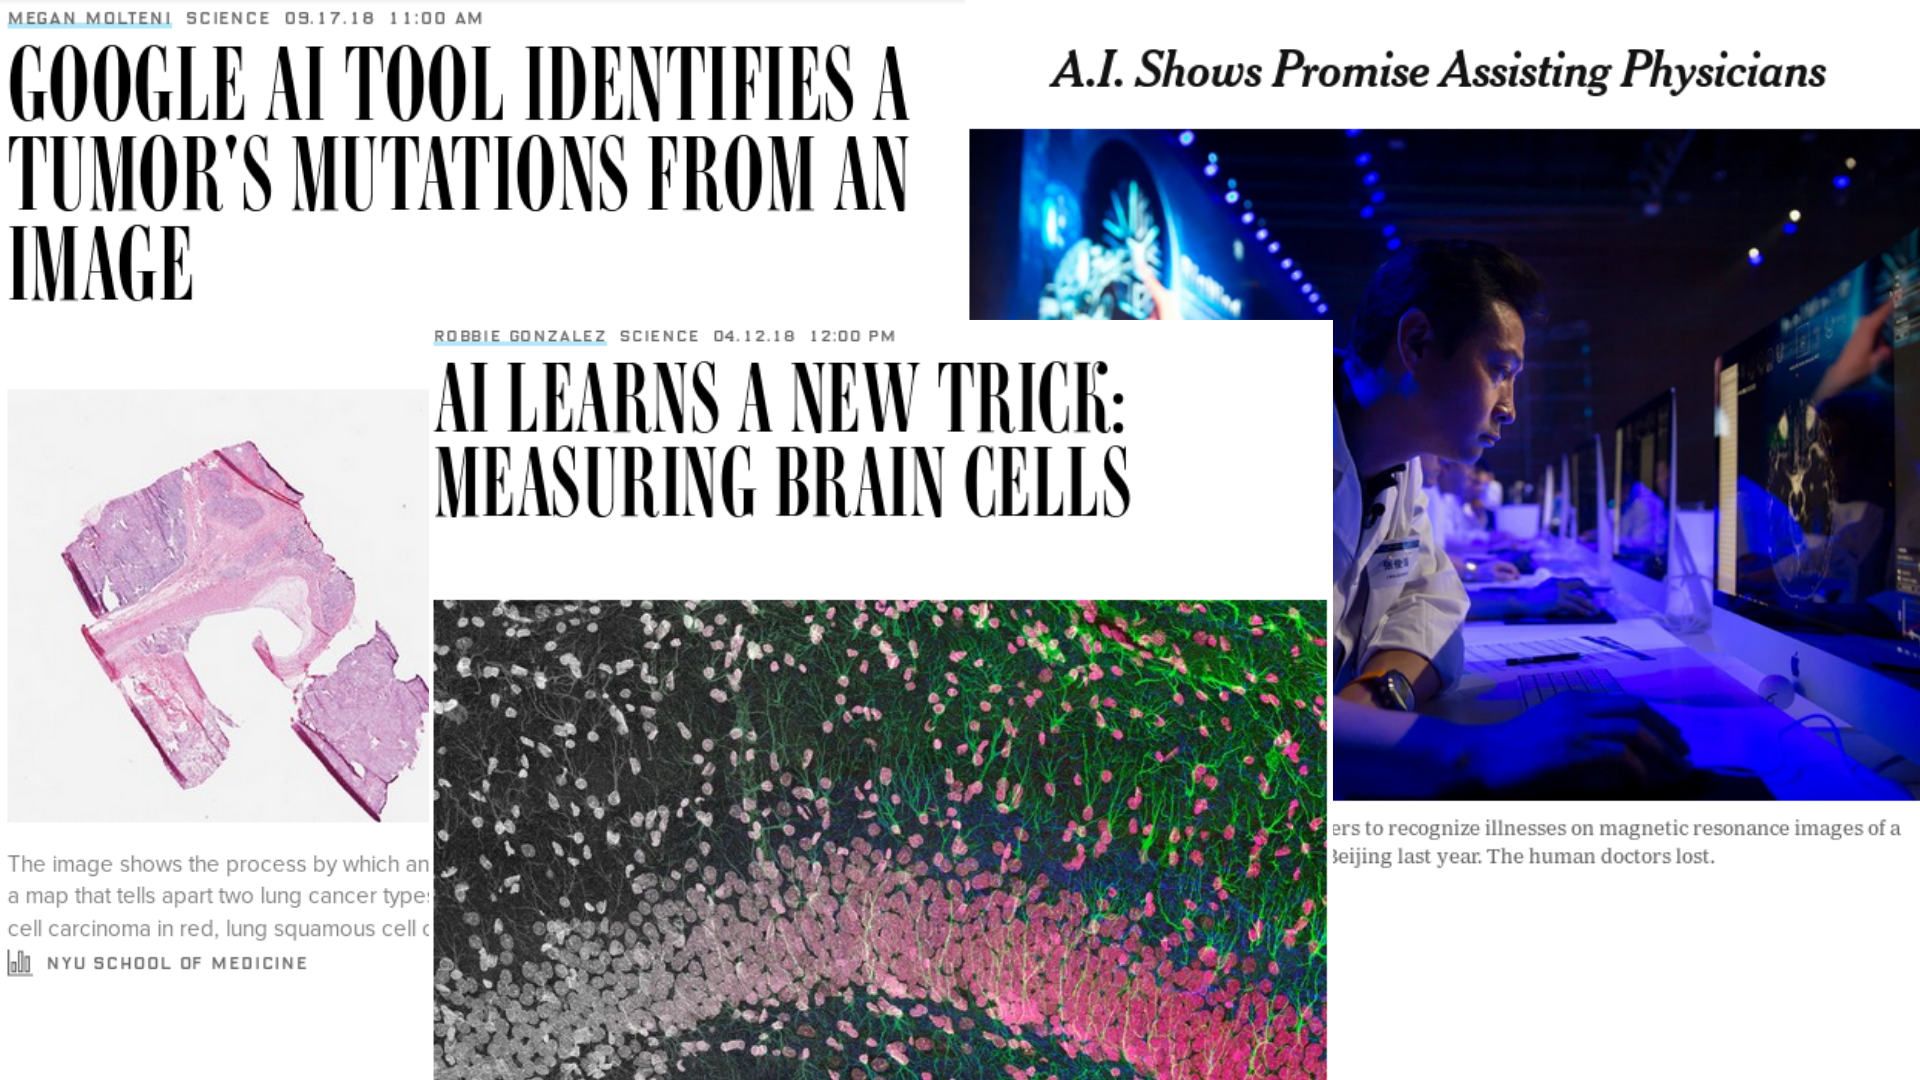
\includegraphics[width=.95\paperwidth]{imgs/news/1}}
  \end{center}
\end{frame}

\begin{frame}
  % \vspace{.6cm}
  \begin{center}
  \makebox[\textwidth]{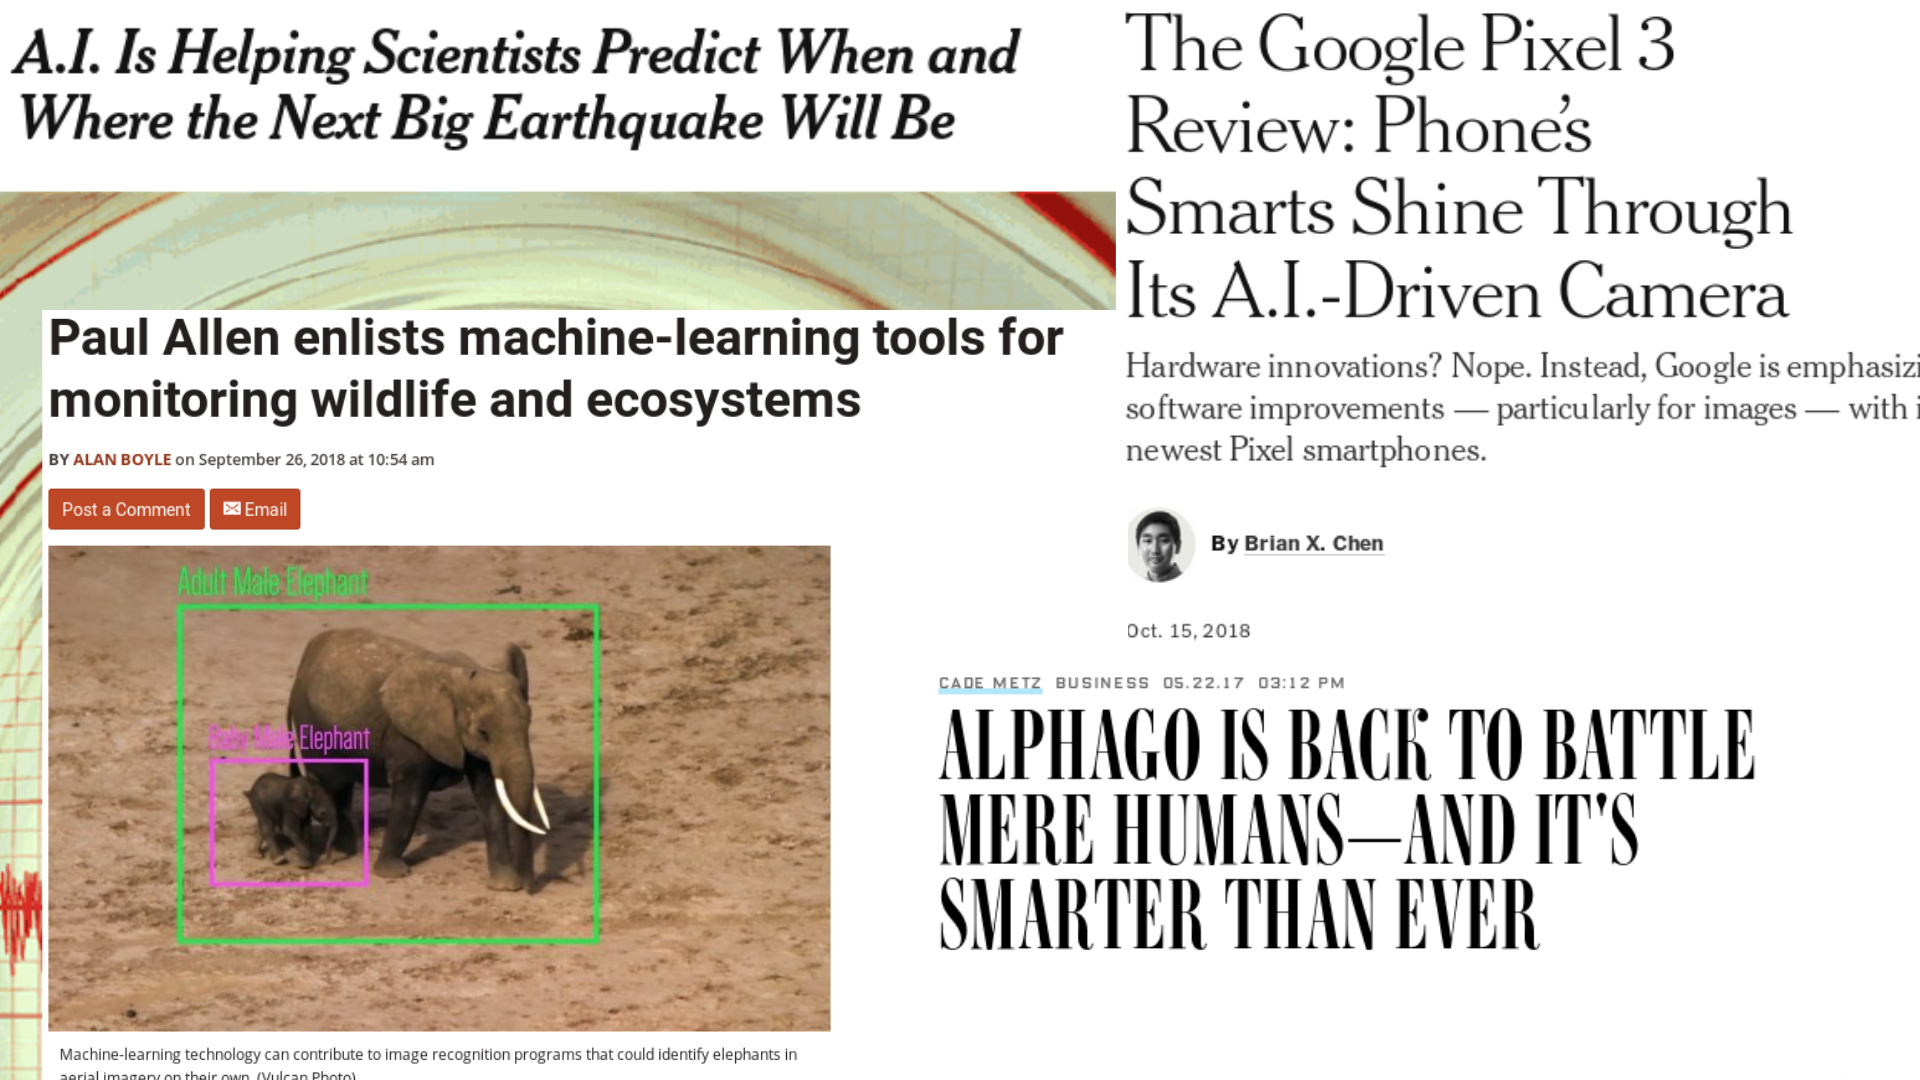
\includegraphics[width=.95\paperwidth]{imgs/news/2}}
  \end{center}
\end{frame}

% AI is the new electricity
\begin{frame}
  \vspace{.6cm}
  \textbf{``AI is the new electricity"} \\
  \qquad \qquad \qquad \small{\textit{Andrew NG}} \\

  \vspace{.6cm}
  \begin{figure}
    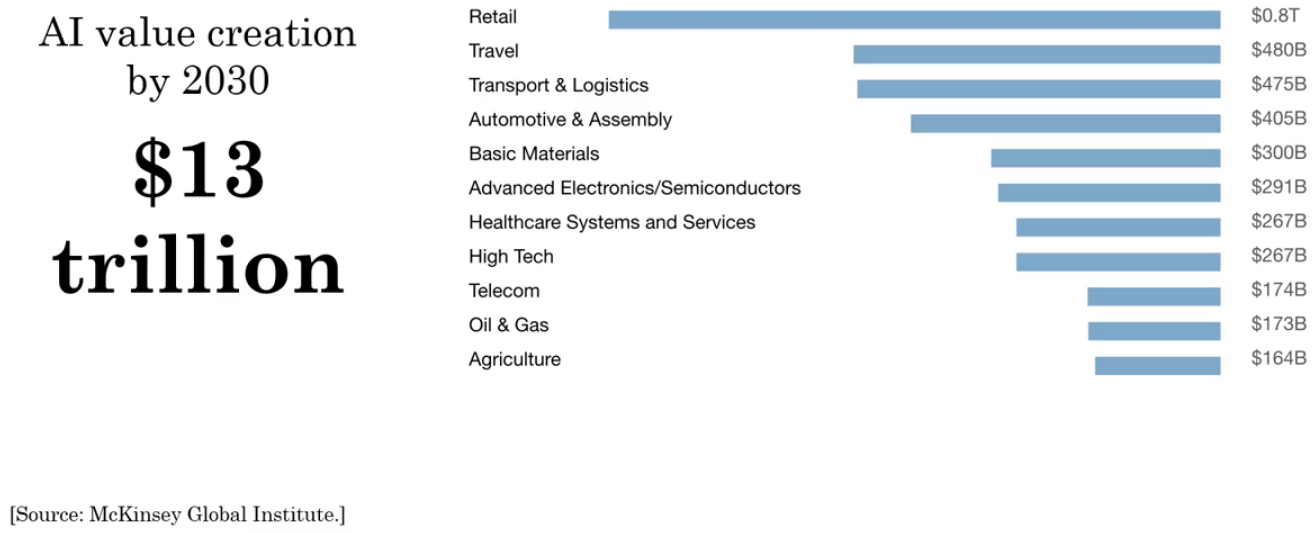
\includegraphics[width=1\linewidth]{imgs/ai_for_everyone_course/1}
  \end{figure}
\end{frame}

% Buzzwords
\begin{frame}
  \vspace{.4cm}

  \begin{figure}
    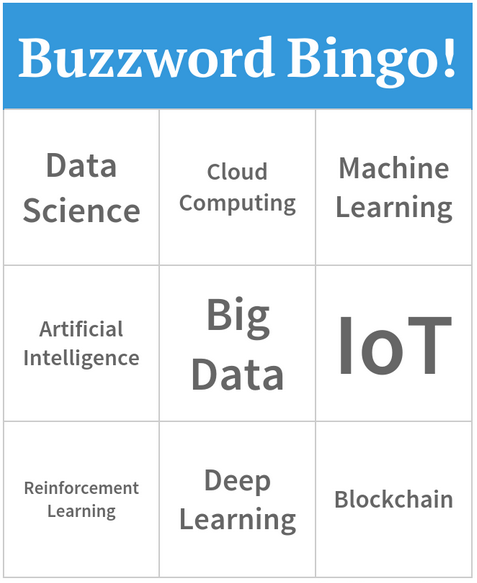
\includegraphics[width=.64\linewidth]{imgs/buzzwords}
  \end{figure}
\end{frame}

% Definitions
\begin{frame}
  \begin{multicols}{2}
  \textbf{Machine Learning}

  ``Field of study that gives computers the ability to learn without being explicitly programmed."

  -Arthur Samuel (1959)

  \columnbreak

  \textbf{Data Science}

  Science of extracting knowledge and insights from data.


  \end{multicols}

  \begin{multicols}{2}
    \textit{An ML projects results in a piece of software that runs.}

    \columnbreak

    \textit{A Data Science projects is often a presentation that summarizes conclusions for executives to take business actions or that summarizes conclusions for a product team to decide how to improve a website.}

  \end{multicols}
\end{frame}

% Definitions
\begin{frame}
  \begin{multicols}{2}
  \textbf{Artificial Intelligence} \\ \hfill \break

  ``the study and design of intelligent agents" where an intelligent agent is a system that perceives its environment and takes actions which maximizes its chances of success.

  \columnbreak

  \begin{figure}
    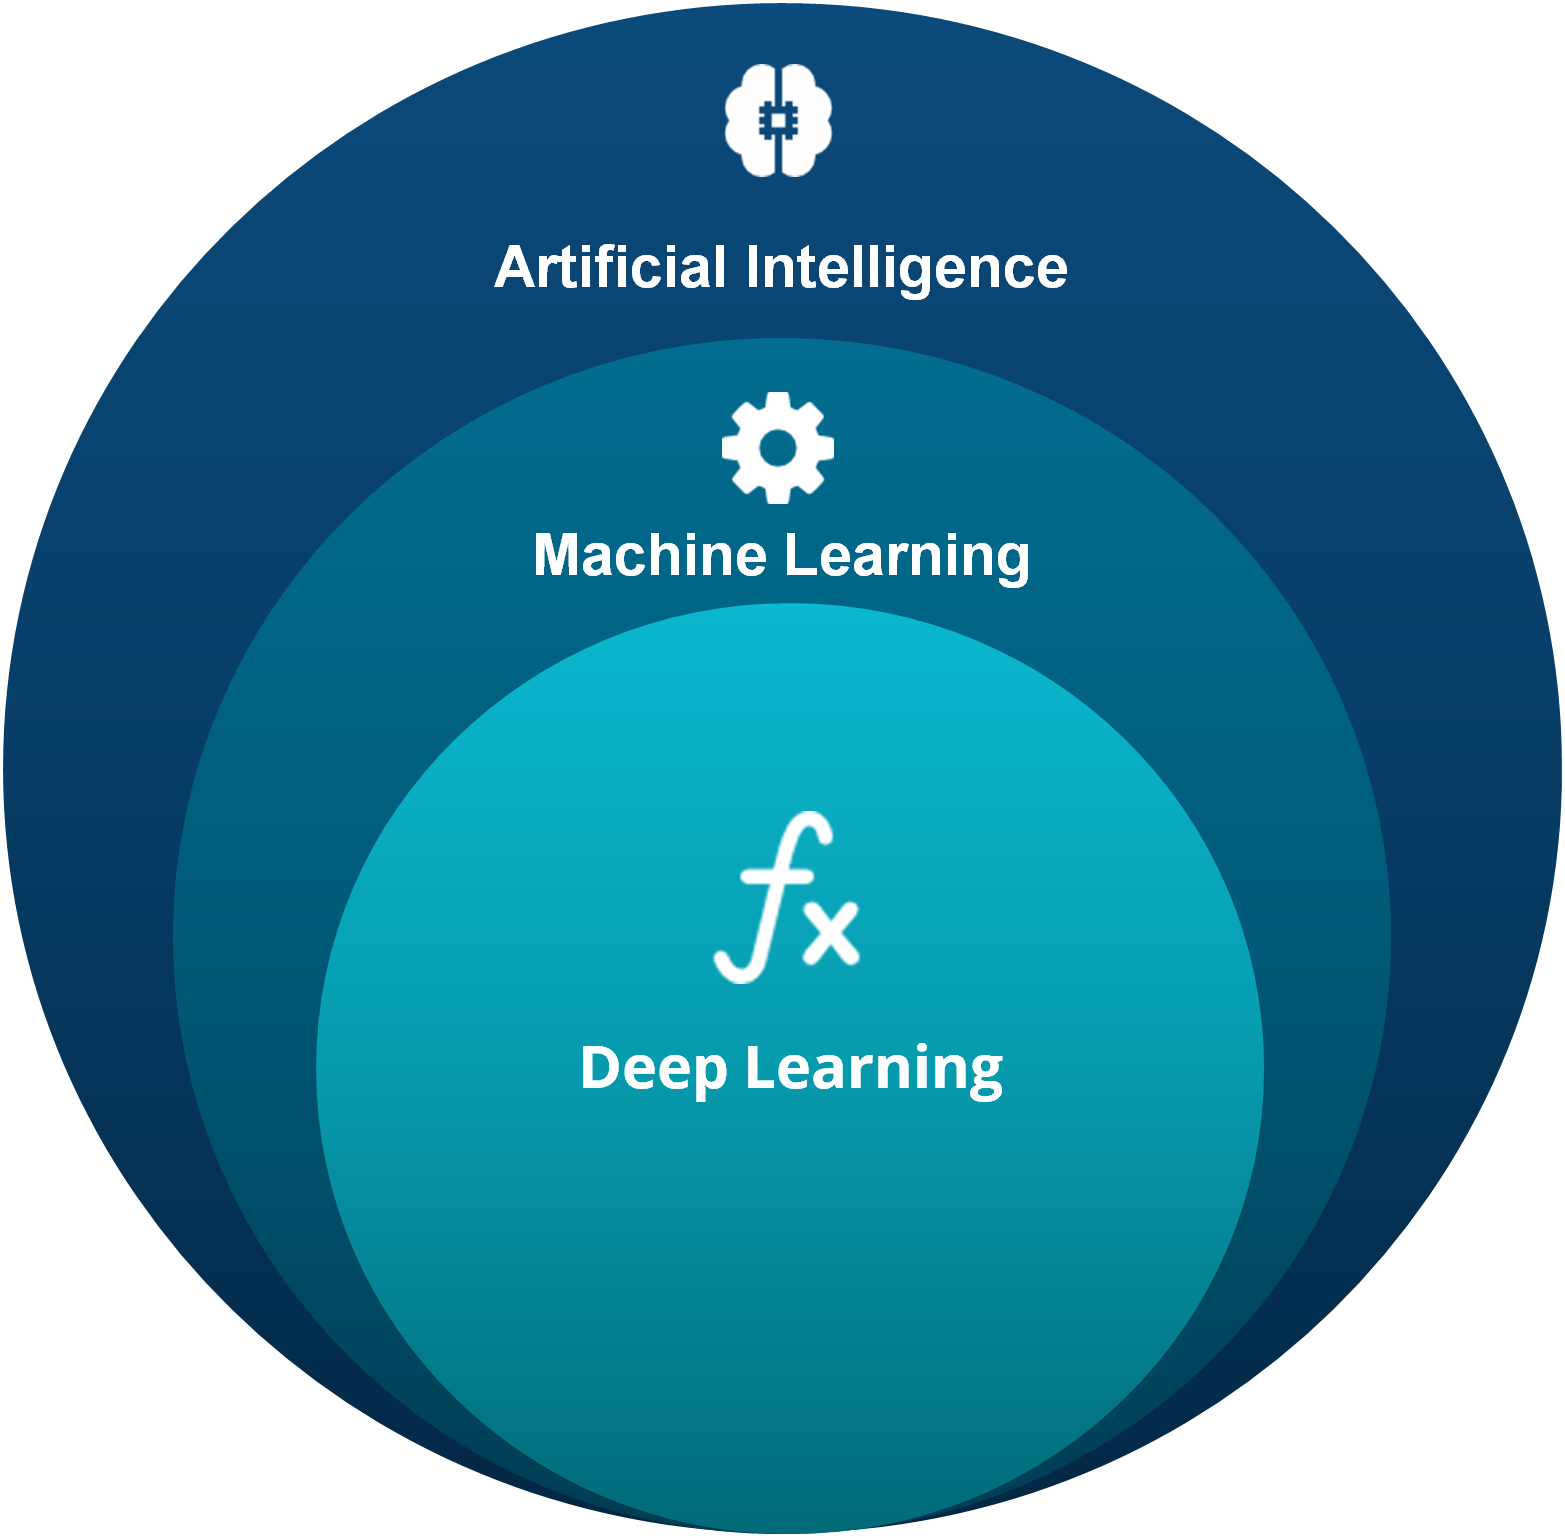
\includegraphics[width=.9\linewidth]{imgs/venn_ai_ml_dl}
  \end{figure}

  \end{multicols}
\end{frame}

\begin{frame}
  \begin{figure}
    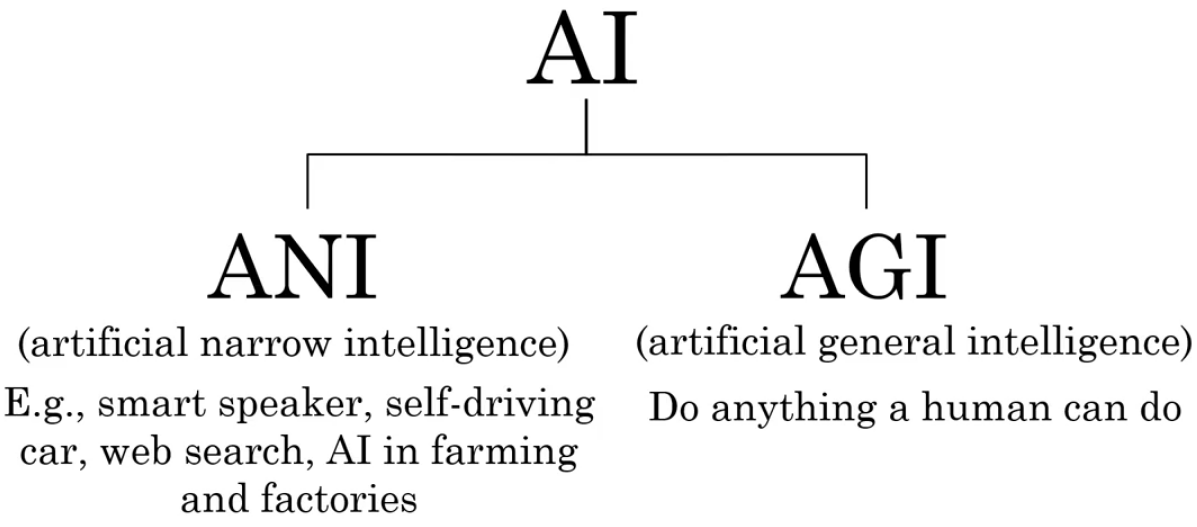
\includegraphics[width=.9\linewidth]{imgs/ai_for_everyone_course/2}
  \end{figure}
\end{frame}

% Color Restoration
\begin{frame}
  \vspace{.6cm}
  \textbf{Color Restoration} [\href{http://iizuka.cs.tsukuba.ac.jp/projects/colorization/data/colorization_sig2016.pdf}{link}] \\
  \small{Automatic colorization and color restoration in black and white images.} \\
  \vspace{.6cm}
  \begin{figure}
    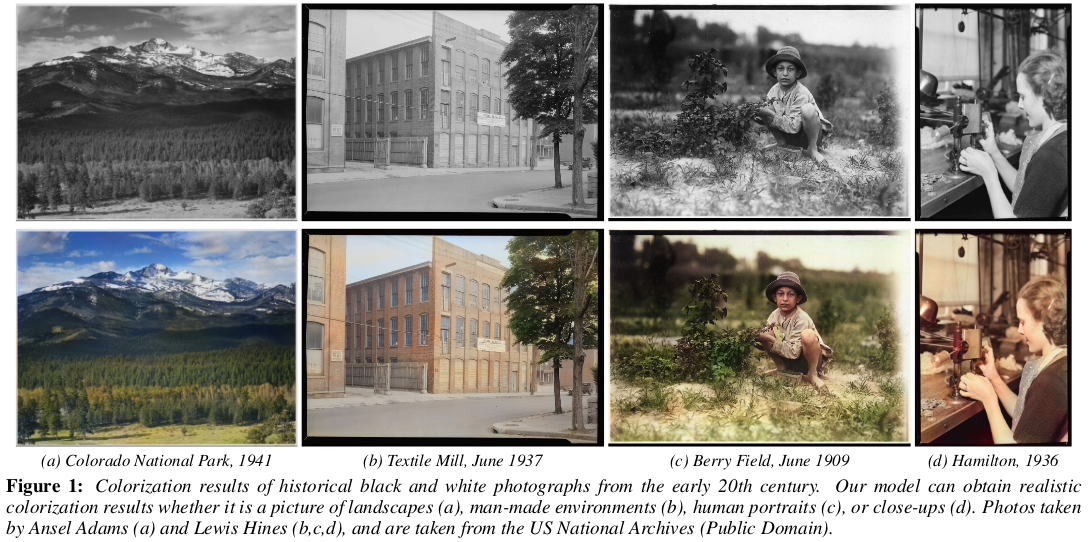
\includegraphics[width=1\linewidth]{imgs/edx_dl_keras/1}
  \end{figure}
\end{frame}

% Speech Reenactment
\begin{frame}
  \vspace{.6cm}
  \textbf{Speech Reenactment} [\href{https://grail.cs.washington.edu/projects/AudioToObama/}{link}] \\
  \small{Synthesizing Obama: Learning Lip Sync from Audio.} \\

  \vspace{.6cm}
  \begin{figure}
    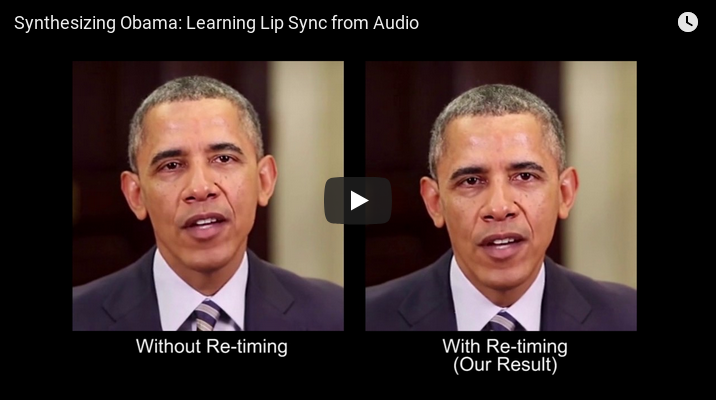
\includegraphics[width=1\linewidth]{imgs/edx_dl_keras/6}
  \end{figure}
\end{frame}

% Diagnose crop diseases
\begin{frame}
  \vspace{.6cm}
  \textbf{Diagnose crop diseases} [\href{https://www.youtube.com/watch?v=NlpS-DhayQA}{link}] \\

  \vspace{.6cm}
  \begin{figure}
    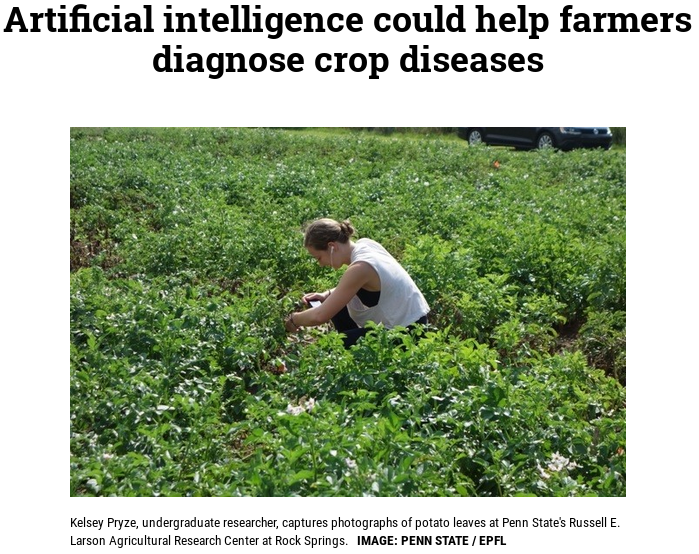
\includegraphics[width=.7\linewidth]{imgs/edx_dl_keras/7}
  \end{figure}
\end{frame}

% Car Vehicle / Traffic Lights / Πedestrian detection with YOLO
\begin{frame}
  \vspace{.6cm}
  \textbf{Car Vehicle / Traffic Lights / Πedestrian detection with YOLO} [\href{https://www.youtube.com/watch?v=OksuVuNY5o0}{link}] \\

  \vspace{.6cm}
  \begin{figure}
    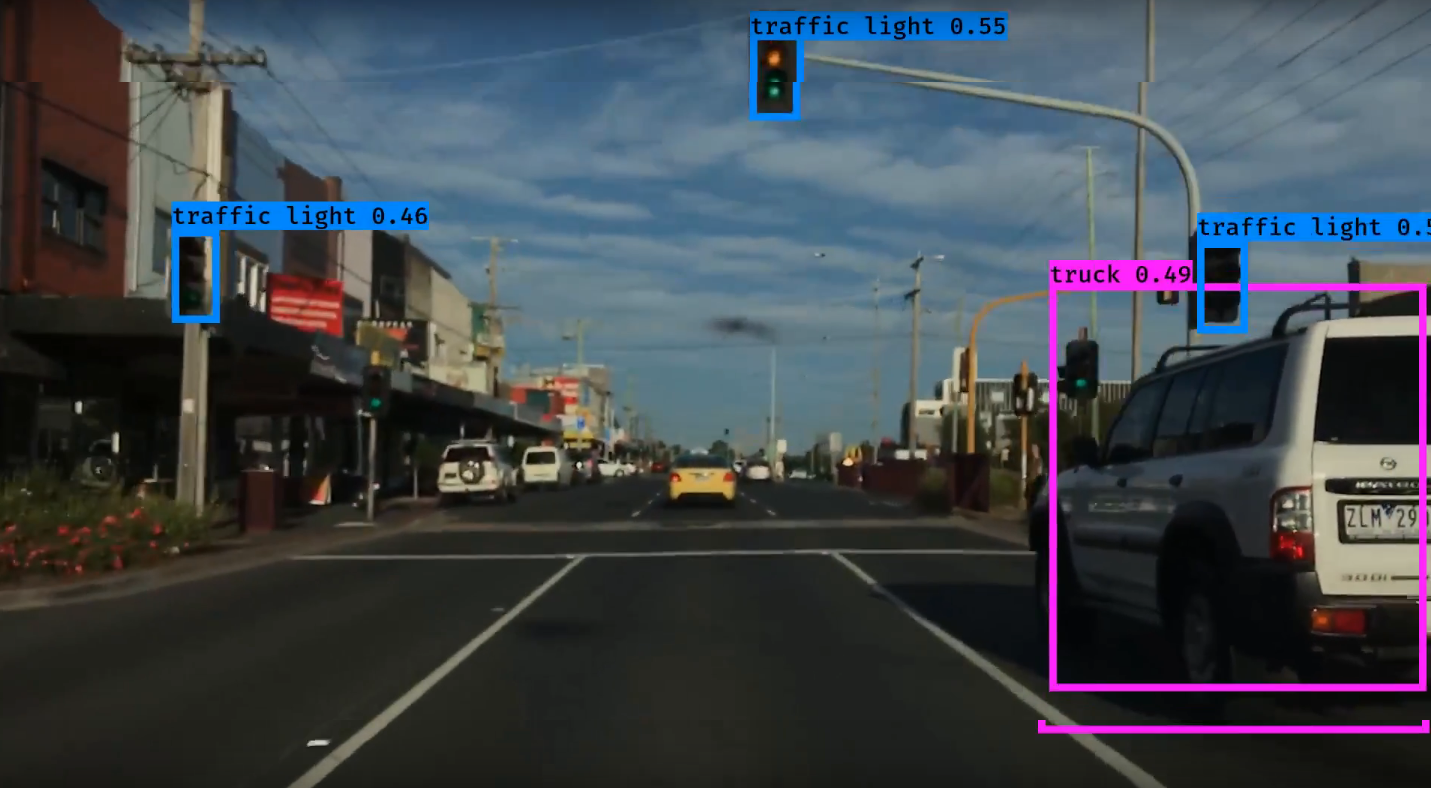
\includegraphics[width=.85\linewidth]{imgs/edx_dl_keras/8}
  \end{figure}
\end{frame}

% NVIDIA Invents AI Interactive Graphics
\begin{frame}
  \vspace{.6cm}
  \textbf{NVIDIA Invents AI Interactive Graphics} [\href{https://news.developer.nvidia.com/nvidia-invents-ai-interactive-graphics/}{link}] \\

  \vspace{.6cm}
  \begin{figure}
    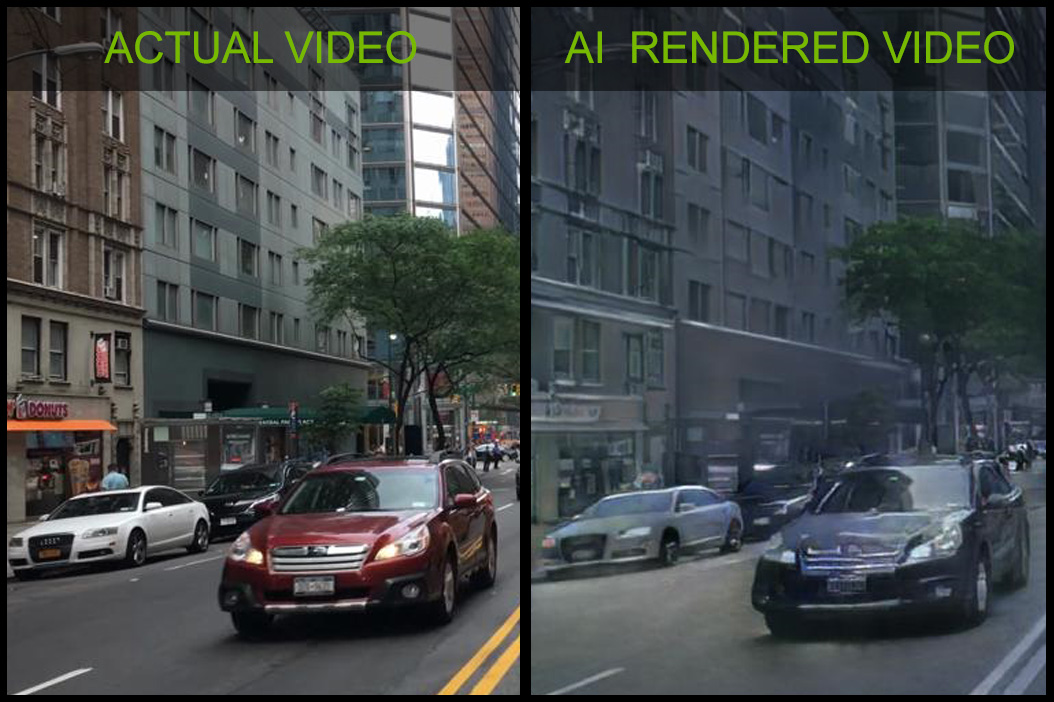
\includegraphics[width=.9\linewidth]{imgs/news/nvidia_1}
  \end{figure}
\end{frame}

% funny_1
\begin{frame}
  \vspace{.6cm}
  \begin{figure}
    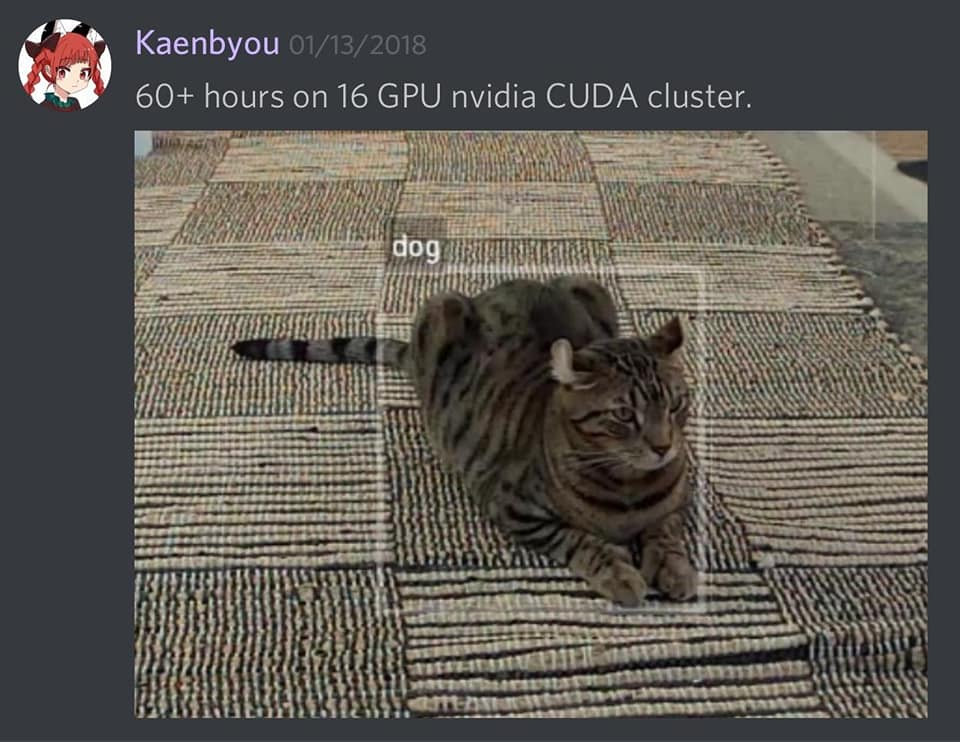
\includegraphics[width=.9\linewidth]{imgs/funny_1}
  \end{figure}
\end{frame}

% funny_2
\begin{frame}
  \vspace{.3cm}
  \begin{figure}
    
\includegraphics[width=.6\linewidth]{imgs/funny_2}
  \end{figure}
\end{frame}

% timeline
\begin{frame}
\begin{figure}
  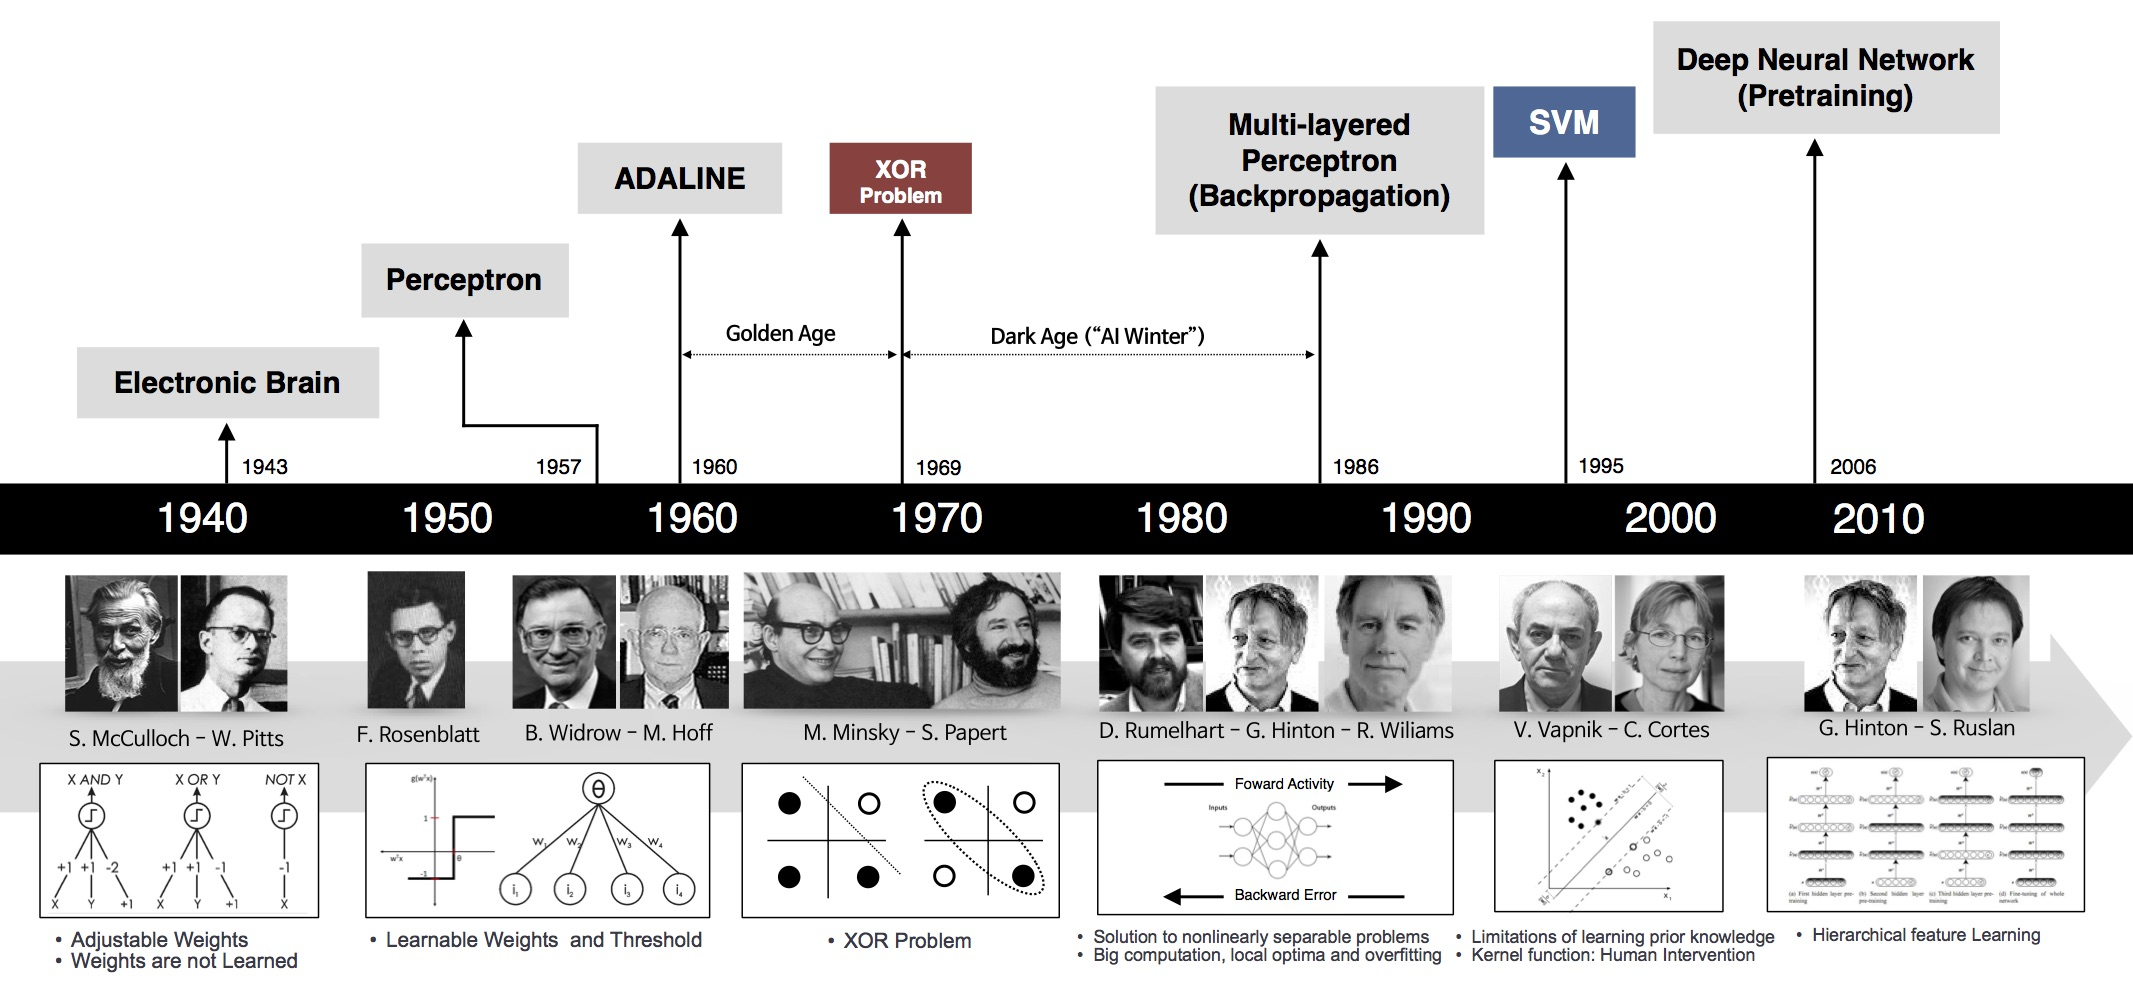
\includegraphics[width=1\linewidth]{imgs/nn_timeline}
\end{figure}
\end{frame}

% Neuron
\begin{frame}
  \vspace*{1cm}
  \textbf{Neuron:} The basic computational unit of the brain  \\
  \textbf{Walter Pitts and Warren McCulloch [1943]:}\\
  \textbf{Thresholded logic unit} (designed to mimic the way a neuron was thought to work) \\
  adjustable but \textit{not learned} weights \\
  \vspace*{-.5cm}
  \begin{eqnarray}
  \mbox{output} & = & \left\{ \begin{array}{ll}
  0 & \mbox{if } \sum_j w_j x_j \leq \mbox{ threshold} \\
  1 & \mbox{if } \sum_j w_j x_j > \mbox{ threshold}
  \end{array} \right.
  \nonumber
  \end{eqnarray}
  \hrulefill \\
  \begin{figure}[ht]
  	\centering
  	\subfloat[Biological Neuron]{%
  		\label{fig:first}%
  		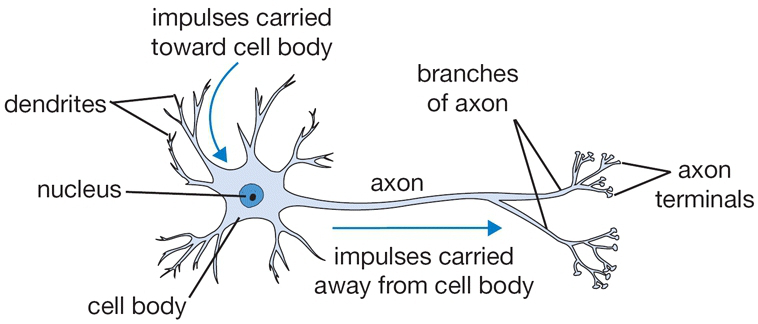
\includegraphics[width=0.5\linewidth]{imgs/neuron}}%
  	\qquad
  	\subfloat[Artificial Neuron]{%
  		\label{fig:second}%
  		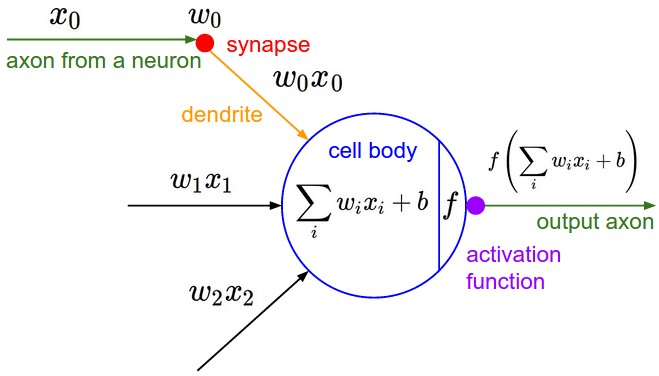
\includegraphics[width=0.4\linewidth]{imgs/artificial_neuron}}
  \end{figure}
\end{frame}

% Thresholded logic unit
\begin{frame}
  \vspace*{1cm}
  \textbf{Thresholded logic unit:} Maps inputs to 1 or 0 \\
  % \begin{multicols}{2}
    \begin{eqnarray}
    \mbox{output} & = & \left\{ \begin{array}{ll}
    0 & \mbox{if } \sum_j w_j x_j \leq \mbox{ threshold} \\
    1 & \mbox{if } \sum_j w_j x_j > \mbox{ threshold}
    \end{array} \right.
    \nonumber
    \end{eqnarray}

    % \columnbreak

    \begin{figure}
      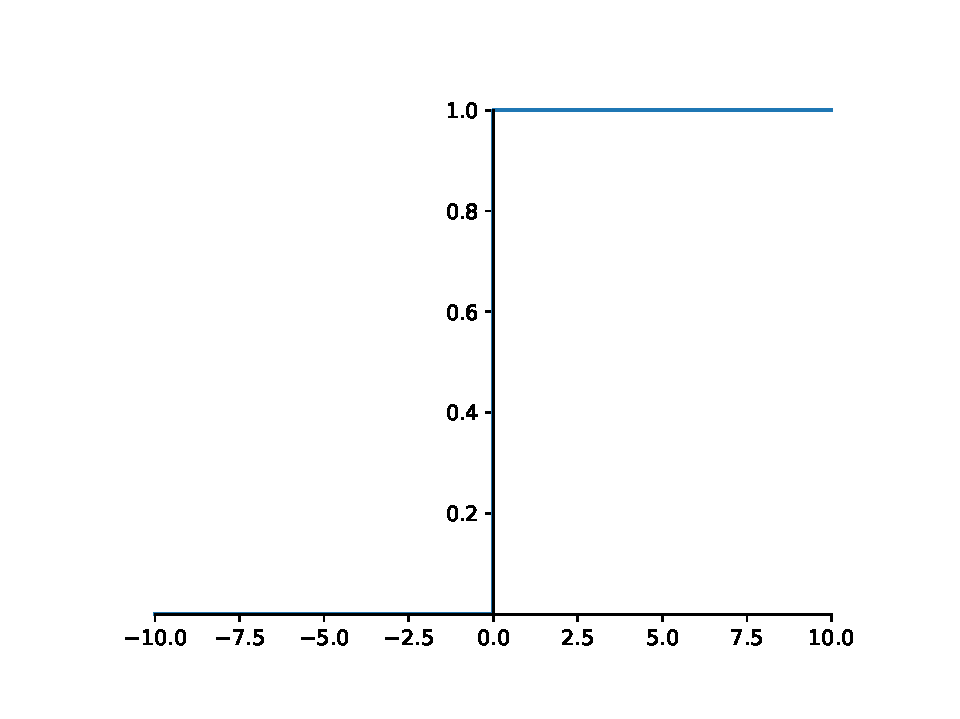
\includegraphics[width=.7\linewidth]{imgs/step.pdf}
    \end{figure}
  % \end{multicols}
\end{frame}

% Frank Rosenblatt’s “perceptron”
\begin{frame}
  \textbf{Frank Rosenblatt’s “perceptron” [1957]:} \\First real precursor to modern neural networks \\
  Developed \textbf{rule for learning weights}

  \vspace{-.5cm}
  \begin{figure}
    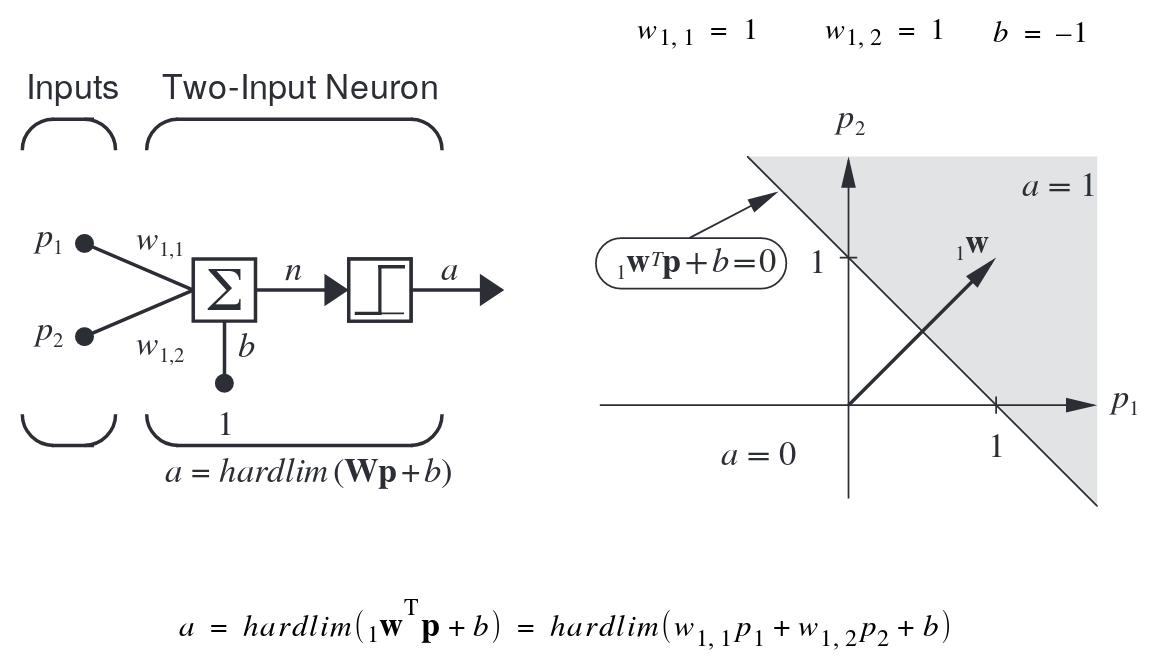
\includegraphics[width=.8\linewidth]{imgs/perceptron_1}
  \end{figure}
  \vspace{-.5cm}
  \textbf{Decision Boundary:} $w_{1,1}p_1 + w_{1,2}p_2 + b = 0$ \\
  \textbf{Linear equation:} $ax + by + c = 0$
\end{frame}

% Example - OR gate
\begin{frame}
  \vspace{1cm}
  \textbf{Supervised Learning} \\
  Network is provided with a set of examples of proper network behavior (inputs/targets)
  $$\{p_1, t_1\}, \{p_2, t_2\}, ..., \{p_Q, t_Q\}$$

  \textbf{Example - OR gate} \\ \hfill \break
  \vspace{-.6cm}
  \begin{figure}
    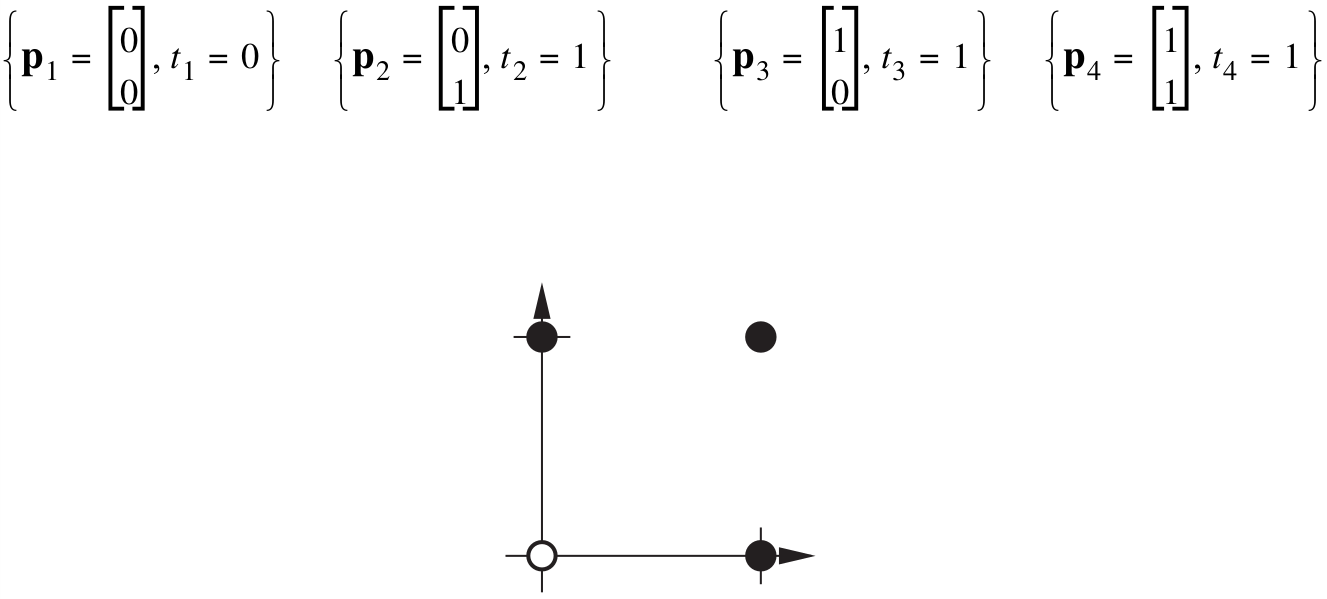
\includegraphics[width=.9\linewidth]{imgs/perceptron_or}
  \end{figure}
\end{frame}

% Example - OR gate
\begin{frame}
  \vspace{1cm}
  \textbf{Example - OR gate}
  \begin{figure}
    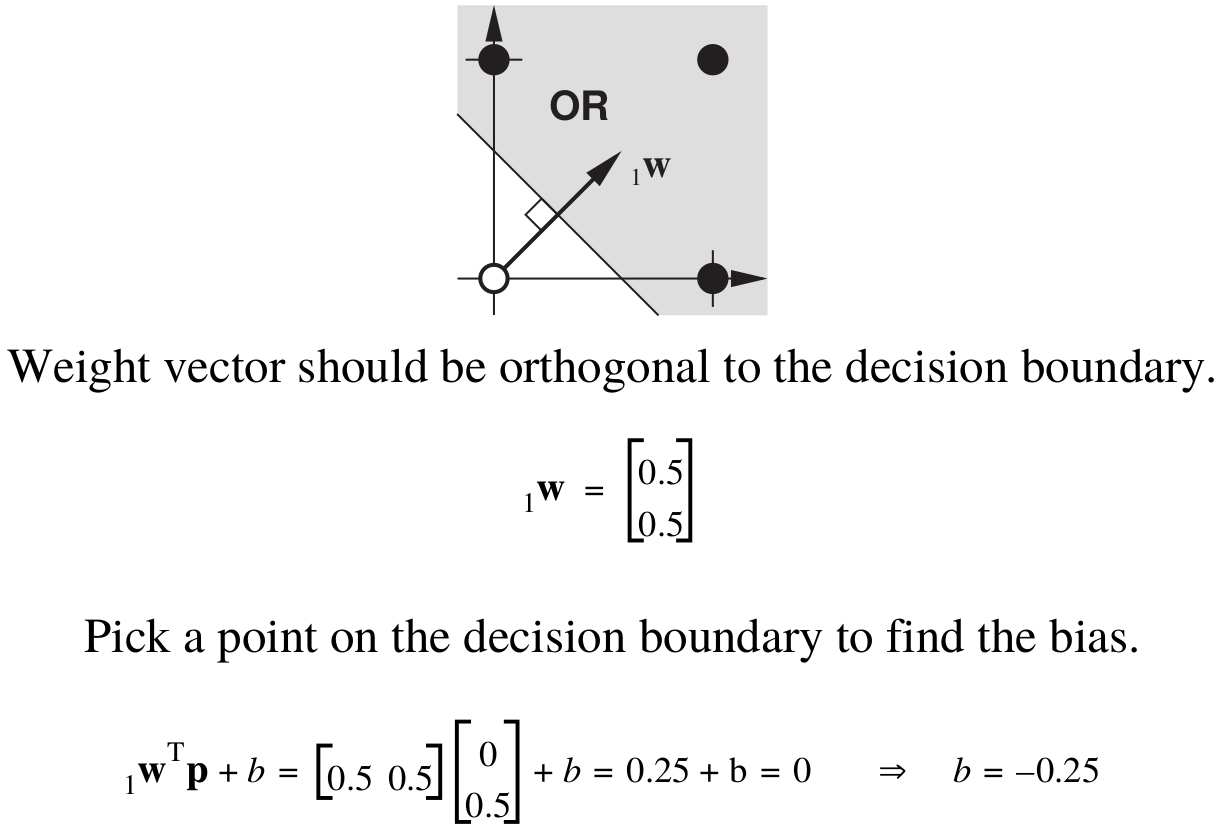
\includegraphics[width=.9\linewidth]{imgs/perceptron_or_2}
  \end{figure}
\end{frame}


\begin{frame}
  \vspace{1cm}
  \textbf{Learning Rule Test Problem}
  \begin{figure}
    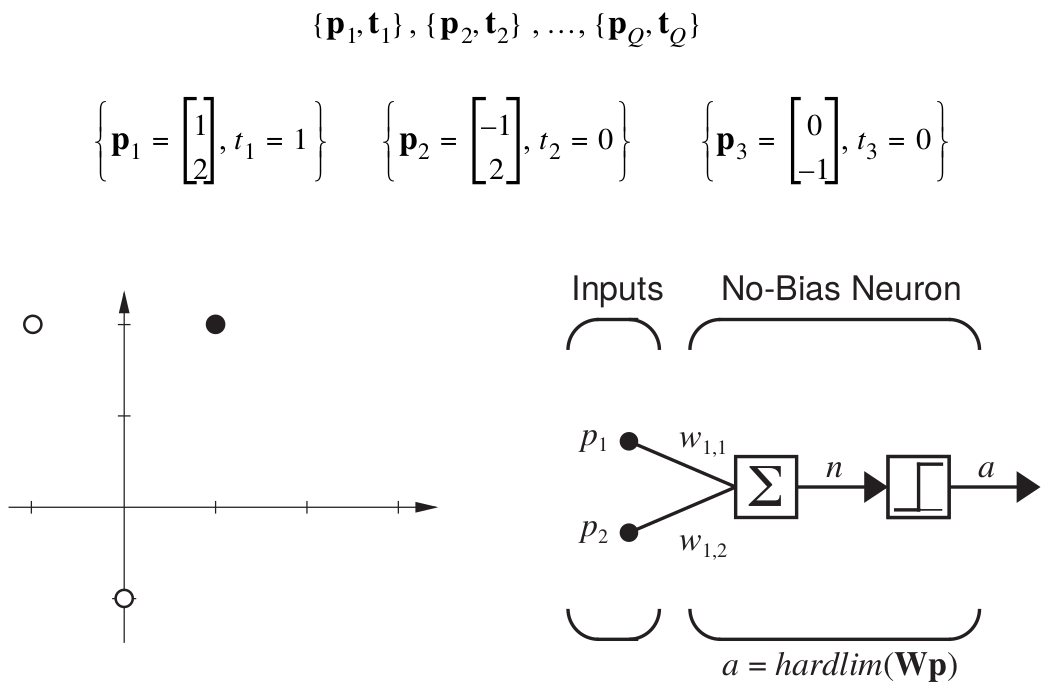
\includegraphics[width=.9\linewidth]{imgs/perceptron_ex_1}
  \end{figure}
\end{frame}

\begin{frame}
  \vspace{1cm}
  \textbf{Starting Point}
  \begin{figure}
    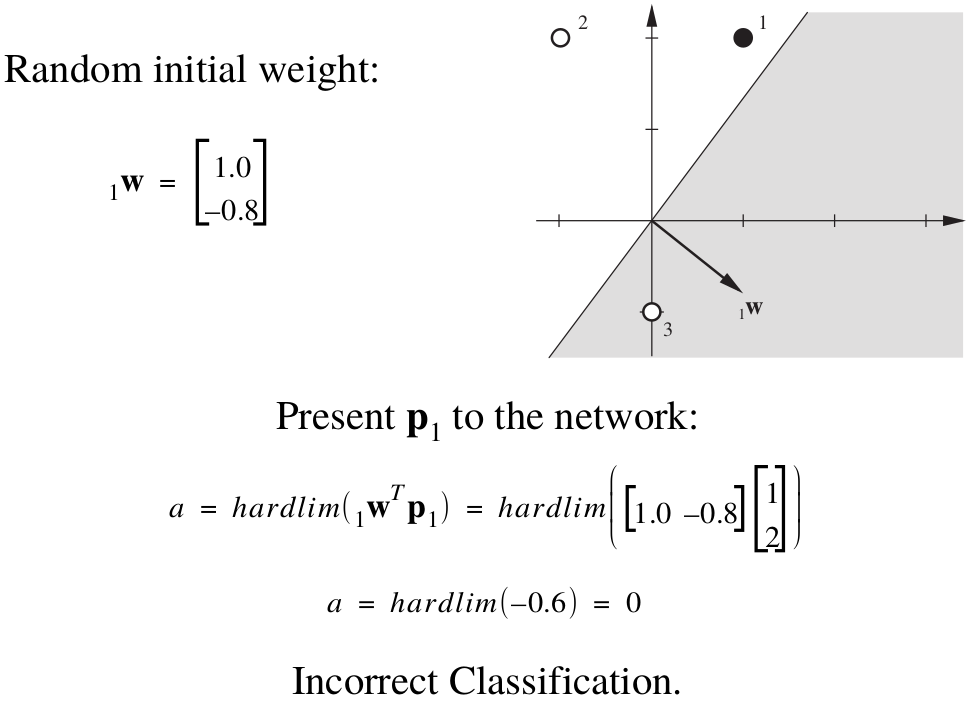
\includegraphics[width=.9\linewidth]{imgs/perceptron_ex_2}
  \end{figure}
\end{frame}

\begin{frame}
  \vspace{1cm}
  \textbf{Tentative Learning Rule}
  \begin{figure}
    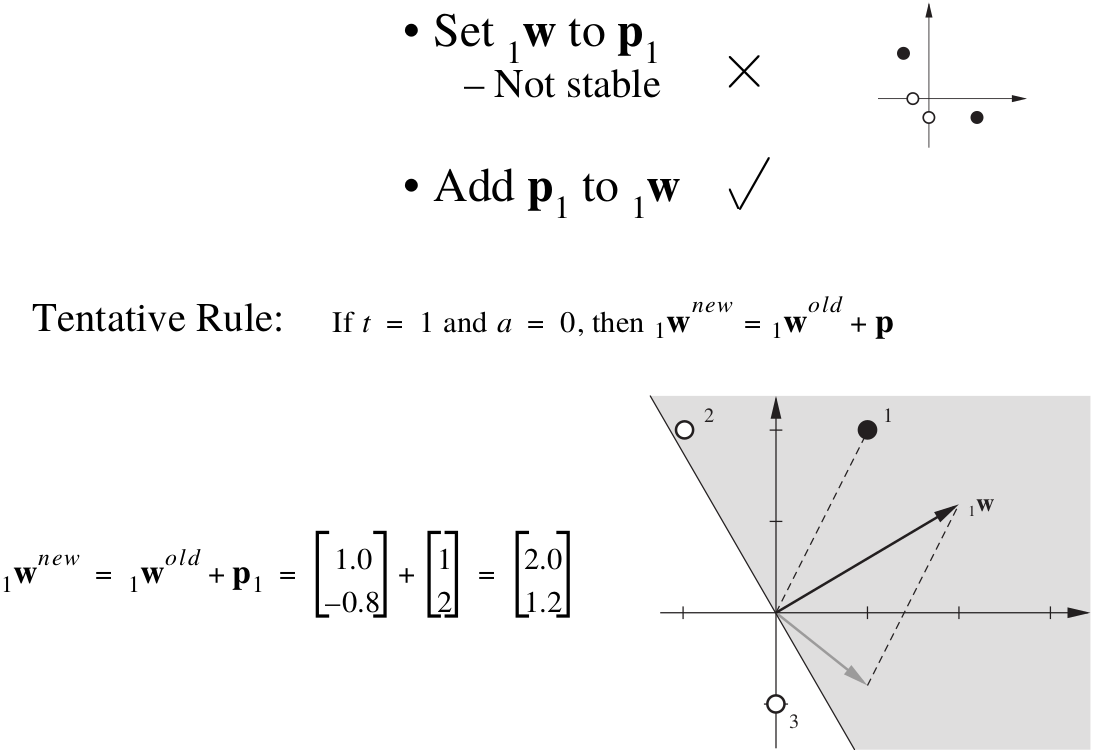
\includegraphics[width=.9\linewidth]{imgs/perceptron_ex_3}
  \end{figure}
\end{frame}

\begin{frame}
  \vspace{1cm}
  \textbf{Second Input Vector}
  \begin{figure}
    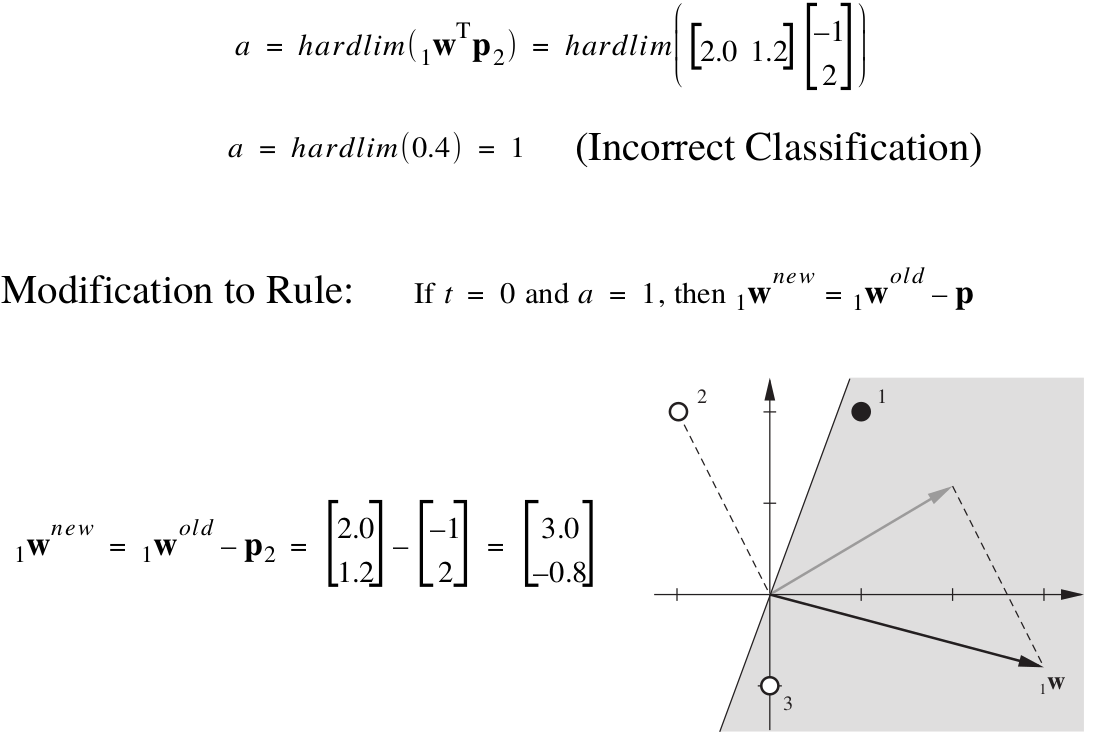
\includegraphics[width=.9\linewidth]{imgs/perceptron_ex_4}
  \end{figure}
\end{frame}

\begin{frame}
  \vspace{1cm}
  \textbf{Third Input Vector}
  \begin{figure}
    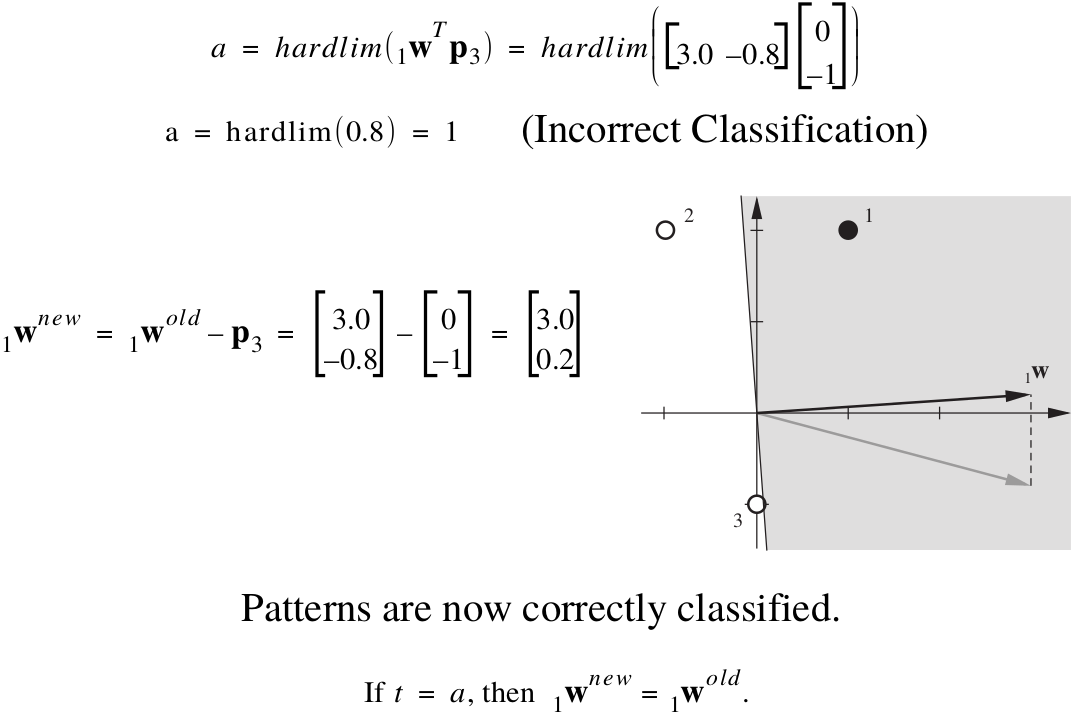
\includegraphics[width=.9\linewidth]{imgs/perceptron_ex_5}
  \end{figure}
\end{frame}

\begin{frame}
  \vspace{.5cm}
  \textbf{Unified Learning Rule}
  \begin{figure}
    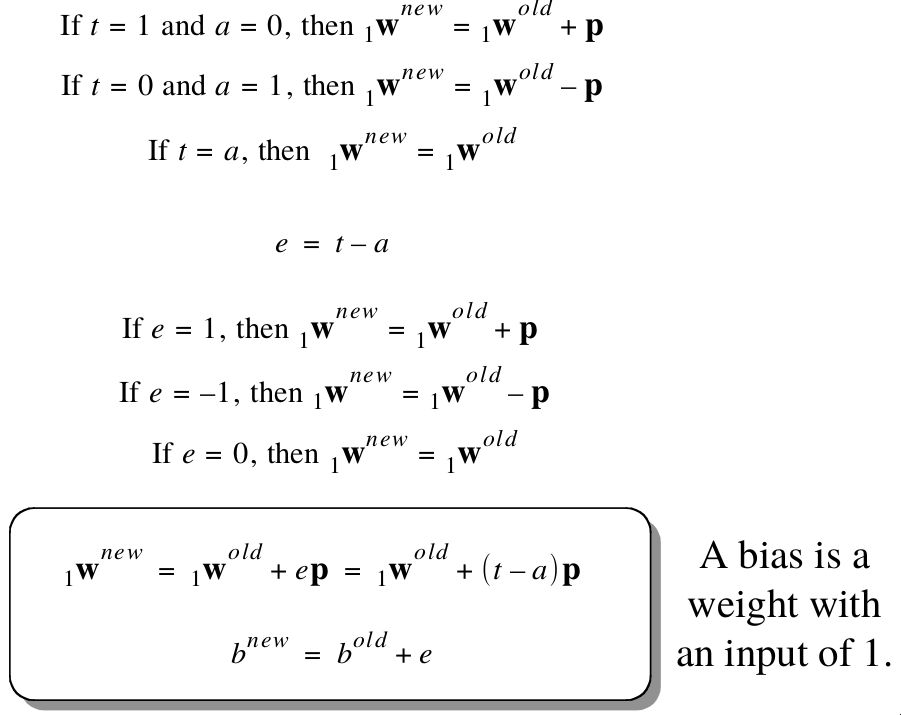
\includegraphics[width=.9\linewidth]{imgs/perceptron_ex_6}
  \end{figure}
\end{frame}

% \begin{frame}
% % $p_2 = -\frac{b}{w_{1,2}}$, if $p_1 = 0$ \qquad
% % $p_1 = -\frac{b}{w_{1,1}}$, if $p_2 = 0$
% \textbf{Perceptron's Learning Rule} \\ \hfill \break
% \centering
% If $t = 1$ and $\alpha = 0$, then $w^{new} = w^{old} + p$ \\
% If $t = 0$ and $\alpha = 1$, then $w^{new} = w^{old} - p$ \\
% If $t = \alpha$, then $w^{new} = w^{old}$ \\
%
% $$e = t - \alpha$$
% If $e = 1$, then $w^{new} = w^{old} + p$ \\
% If $e = -1$, then $w^{new} = w^{old} - p$ \\
% If $e = 0$, then $w^{new} = w^{old}$ \\ \hfill \break
%
% $w^{new} = w^{old} + ep = w^{old} + (t-\alpha)p$ \\
% $b^{new} = b^{old} + e$
%
% \end{frame}

\begin{frame}
  % \textbf{AND gate example} \\
  %
  % \[
  % p_1 =
  % \begin{bmatrix}
  %   0 \\
  %   0
  % \end{bmatrix}
  % , t_1 = 0
  % \quad
  % p2 =
  % \begin{bmatrix}
  %   0 \\
  %   1
  % \end{bmatrix}
  % , t_2 = 0 \quad
  % p_3 =
  % \begin{bmatrix}
  %   1 \\
  %   0
  % \end{bmatrix}
  % , t_3 = 0
  % \quad
  % p4 =
  % \begin{bmatrix}
  %   1 \\
  %   1
  % \end{bmatrix}
  % , t_4 = 1\]
  % \vspace{1cm}
  \textbf{Perceptron convergence theorem} \\ \hfill \break
  \textit{The perceptron learning rule will converge to a weight vector (not necessarily unique) that  gives  the  correct  response  for  all  training  patterns,  and it will do so in a finite number of steps.} \\ \hfill \break
  Rosenblatt was so confident that the perceptron would lead to true AI, that in 1959 he remarked: \\ \hfill \break
  \textit{[The perceptron is] the embryo of an electronic computer that [the Navy] expects will be able to walk, talk, see, write, reproduce itself and be conscious of its existence.}

\end{frame}


\begin{frame}

\vspace*{.5cm}
\textbf{Marvin Minsky and Seymor Papert - XOR problem [1969]} \\ \hfill \break
They showed that the perceptron was incapable of learning the simple exclusive-or (XOR) function. \\
They proved that it was theoretically impossible for it to learn such a function, no matter how long you let it train.\\

\textit{(this isn’t surprising to us, as the model implied by the perceptron is a linear one and the XOR function is nonlinear)} \\\hfill \break
At the time this was enough to kill all research on neural nets\\

% Along with the double-PhD wielding Seymor Papert, Minksy wrote a book entitled Perceptrons that effectively killed the perceptron, ending embryonic idea of a neural net. They showed that the perceptron was incapable of learning the simple exclusive-or (XOR) function. Worse, they proved that it was theoretically impossible for it to learn such a function, no matter how long you let it train. Now this isn’t surprising to us, as the model implied by the perceptron is a linear one and the XOR function is nonlinear, but at the time this was enough to kill all research on neural nets \\

\end{frame}

\begin{frame}
  \vspace{.5cm}
  \begin{figure}
    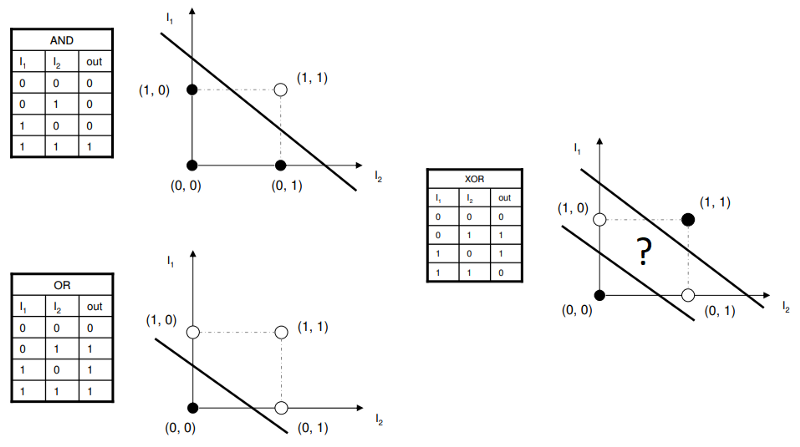
\includegraphics[width=1\linewidth]{imgs/xor_1}
  \end{figure}
\end{frame}

% AI Winter
\begin{frame}
  \vspace{.5cm}
  \begin{figure}
    
\includegraphics[width=.7\linewidth]{imgs/ai_winter}
  \end{figure}
\end{frame}

% XOR Solution???
\begin{frame}
  \vspace{.5cm}
  \centering
  \textbf{\Large{XOR Solution???}}
\end{frame}

% XOR Solution
\begin{frame}
  One single perceptron neuron: One decision boundary (hyperplane) \\
  Two perceptron neurons: Two decision boundaries \\
  \textbf{Multi Layer Perceptron (MLP)}

  \begin{multicols}{2}
    \begin{figure}
      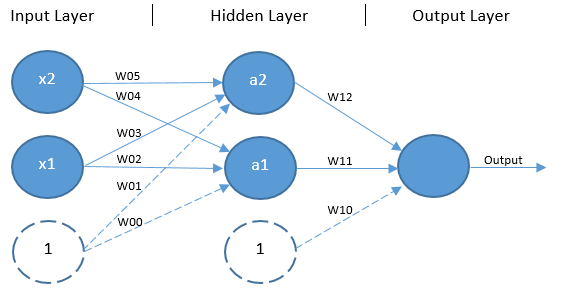
\includegraphics[width=1.2\linewidth]{imgs/mlp_1}
    \end{figure}

    \columnbreak

    \hfill \break
    \begin{figure}
      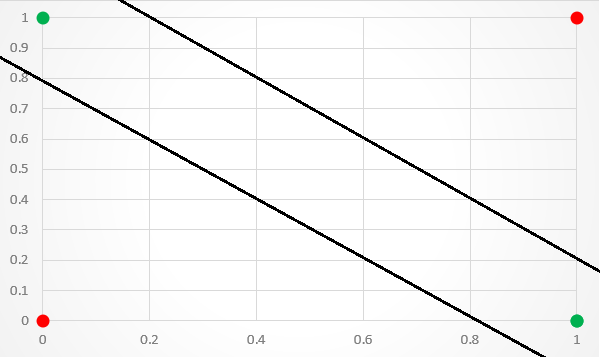
\includegraphics[width=.7\linewidth]{imgs/mlp_1b}
    \end{figure}
  \end{multicols}
\end{frame}

% MLP - XOR as a logic gates
\begin{frame}
  \textbf{As a logic gates}

  \begin{multicols}{2}
    \begin{figure}
      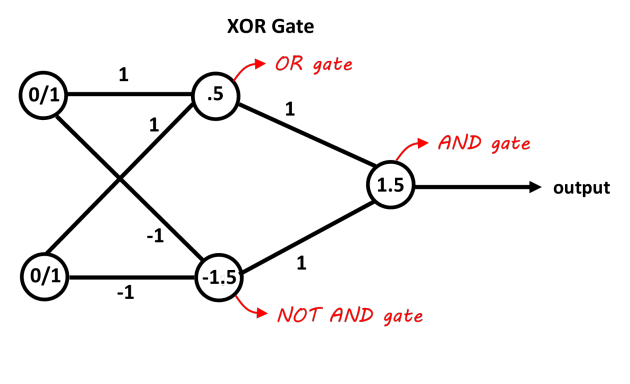
\includegraphics[width=1.2\linewidth]{imgs/mlp_2}
    \end{figure}

    \columnbreak

    \hfill \break
    \begin{figure}
      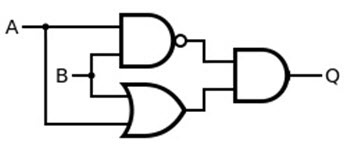
\includegraphics[width=.7\linewidth]{imgs/xor_nand_or}
    \end{figure}
  \end{multicols}
\end{frame}

\begin{frame}
   A network of perceptrons can be used to simulate a circuit containing many NAND gates. And because NAND gates are universal for computation, it follows that perceptrons are also universal for computation. \\ \hfill \break
  \textit{In the mathematical theory of artificial neural networks, the universal approximation theorem states that a feed-forward network with a single hidden layer containing a finite number of neurons can approximate continuous functions on compact subsets of $R^n$, under mild assumptions on the activation function. The theorem thus states that simple neural networks can represent a wide variety of interesting functions when given appropriate parameters}
\end{frame}

\begin{frame}
  \vspace{.8cm}
  \textbf{The problem:} There was no equally powerfull rule (to the Perceptron's) for learning in networks with hidden units. \\
  \vspace{.5cm}

  \textbf{David. Rumelhard, Geoffrey. Hinton and Ronald. Williams - Learning Representations by back-propagating errors [1986]} \\
  (aka ``Backpropagation") \\

  \vspace{.5cm}
  \textbf{Perceptron's delta rule:} $\Delta_pw_{ji} = \eta (t_{pj} - o_{pj})i_{pi} = \eta \delta_{pj} i_{pi}$ \\ \hfill \break
  \textbf{How was this rule derived?} \\
  \textit{For linear units, this rule minimizes the squares of the differences between the actual and the desired output values summed over the output units and all pairs of input/output vectors.} $E = \sum E_p$
  $$ E_p = \frac{1}{2}\sum_j (t_{pj} - o_{pj})^2$$

\end{frame}

\begin{frame}
  \vspace{.5cm}
  \textbf{We have:} input and target data, network architecture \\
  \textbf{We want:} an algorithm which lets us find weights and biases so that the output from the network approximates y(x) (target $t$) for all training inputs x.  To quantify how well we're achieving this goal we define a cost function.

  $$ C(w, b) = \frac{1}{2n}\sum_x (t-\alpha)^2$$
  \textbf{$w$} the collection of all weights in the network, \textbf{$b$} all the biases, \textbf{$n$} the total number of training inputs, \textbf{$\alpha$} is the vector of outputs from the network when \textbf{$x$} is input, and the sum is over all training inputs, \textbf{$x$}.

  The output $\alpha$ depends on $x, w$ and $b$. \\
  We'll call $C$ the quadratic cost function (or mean squared error - MSE).

  $C(w,b)$ is non-negative. \\
  $C(w,b)$ becomes small i.e $C(w,b) \approx 0$ when $t \approx \alpha$.
\end{frame}

\begin{frame}

  $$ C(w, b) = \frac{1}{2n}\sum_x (t-\alpha)^2$$

  $ y = 2x + 4$ \\
  $x = [1, 2, 3, 4, 5, 6, 7, 8]$ \\
  $t = [6, 8, 10, 12, 14, 16, 18, 20]$ \\

  For $w = 3, b = 2$. \\
  $\alpha = [5, 8, 11, 14, 17, 20, 23, 26]$ \\ \hfill \break
  $C(w, b) = \frac{(6-5)^2 + (8-8)^2 + (10-11)^2 + ... + (20-26)^2}{16} = 5.75$ \\ \hfill \break

  The aim of our training algorithm will be to minimize the cost C(w,b) as a function of the weights and biases. In other words, we want to find a set of weights and biases which make the cost as small as possible. We'll do that using an algorithm known as \textbf{gradient descent}.
\end{frame}

\begin{frame}
   Minimize some function, C(v) \\
   it helps to imagine C as a function of just two variables, which we'll call v1 and v2

   \begin{multicols}{2}
     This our function as a kind of a valley!!! \\
     and imagine a ball rolling down the slope of the valley.

     \begin{eqnarray}
     \Delta C \approx \frac{\partial C}{\partial v_1} \Delta v_1 +
     \frac{\partial C}{\partial v_2} \Delta v_2
     \nonumber
     \end{eqnarray}

     \begin{eqnarray}
     \Delta C \approx \nabla C \cdot \Delta v
     \label{eq:2.8}
     \nonumber
     \end{eqnarray}


     \columnbreak
     \begin{figure}
       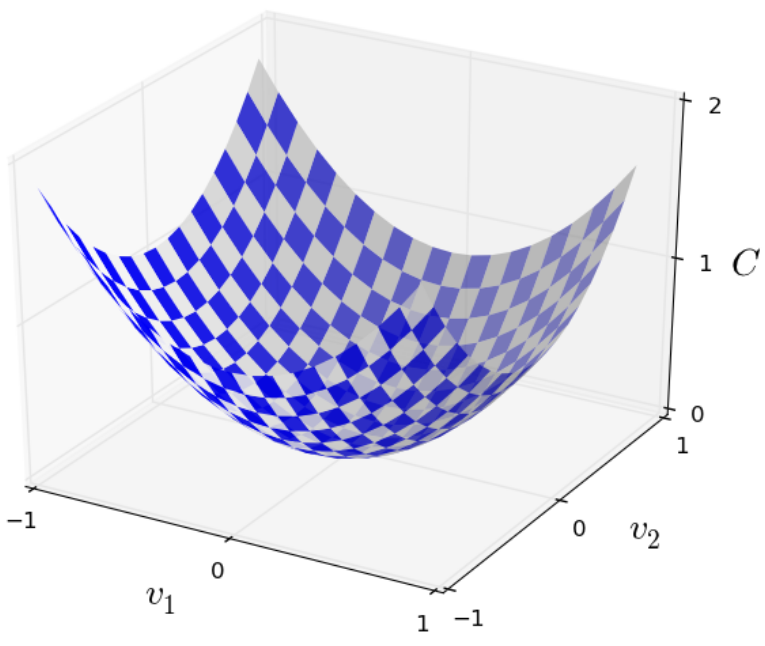
\includegraphics[width=1\linewidth]{imgs/gd_1}
     \end{figure}
  \end{multicols}
\end{frame}

\begin{frame}
  \begin{multicols}{2}
    Choose $\Delta v$ so as to make $\Delta C$ negative: \\

    $\Delta v = -\eta \nabla C$ \\
    $\Delta C \approx - \eta \| \nabla C \| ^2$ \\
    $\Delta C \leq 0$ i.e., $C$ will always decrease,

    $ v \rightarrow v' = v - \eta \nabla C$

  \columnbreak

    \begin{figure}
      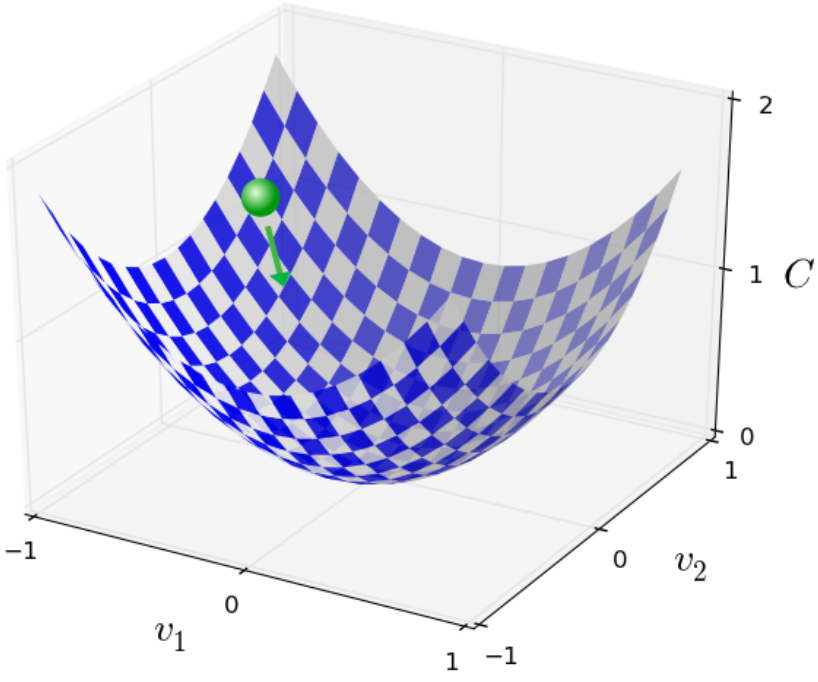
\includegraphics[width=1\linewidth]{imgs/gd_2}
    \end{figure}
  \end{multicols}
\end{frame}

\begin{frame}
  \vspace{1cm}
  % \centering
  \begin{multicols}{2}
  $y = 2x + 4 = wx + b$.\\
  $ C(w, b) = \frac{1}{2n}\sum_x (t-\alpha)^2$

  $\frac{\partial C(w, b)}{\partial b} = \frac{1}{n}\sum(t - (wx + b))$ \\ \hfill \break
  $\frac{\partial C(w, b)}{\partial w} = \frac{1}{n}\sum(t - (wx + b)) \cdot x$ \\ \hfill \break

  $b' = b - \eta \frac{\partial C(w, b)}{\partial b}$ \\
  $w' = w - \eta \frac{\partial C(w, b)}{\partial w}$

  \columnbreak

  \begin{figure}
    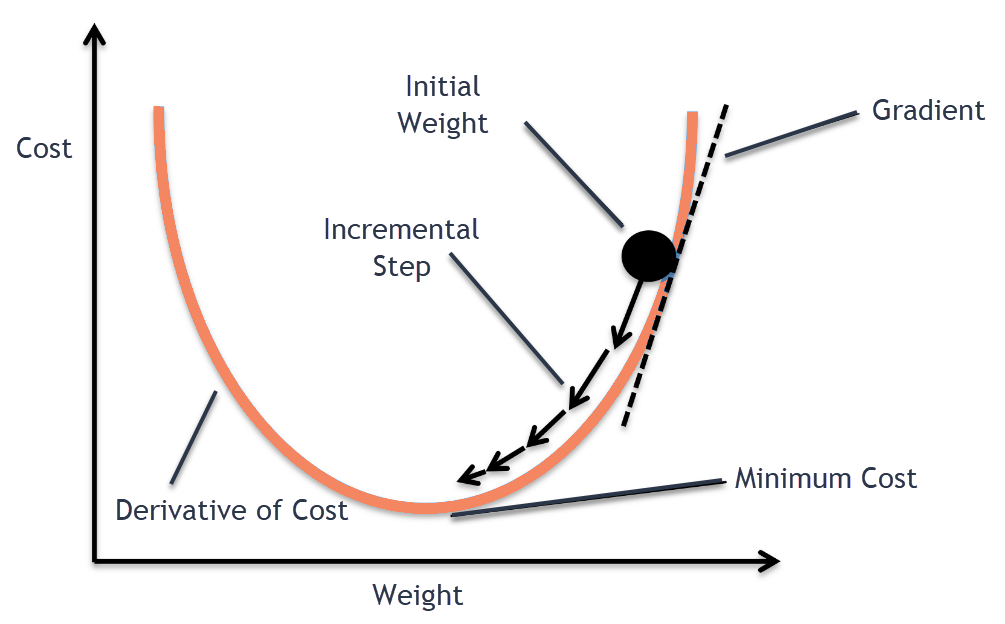
\includegraphics[width=1\linewidth]{imgs/gd_3}
  \end{figure}
  \end{multicols}
\end{frame}

\begin{frame}
  \textbf{So, how do we train a Multi Layer Perceptron?} \\
  \Large{$w_{1.1}^{new} = w_{1.1}^{old} - \eta \frac{\partial C}{\partial w_{1.1}}$}
  \begin{figure}
    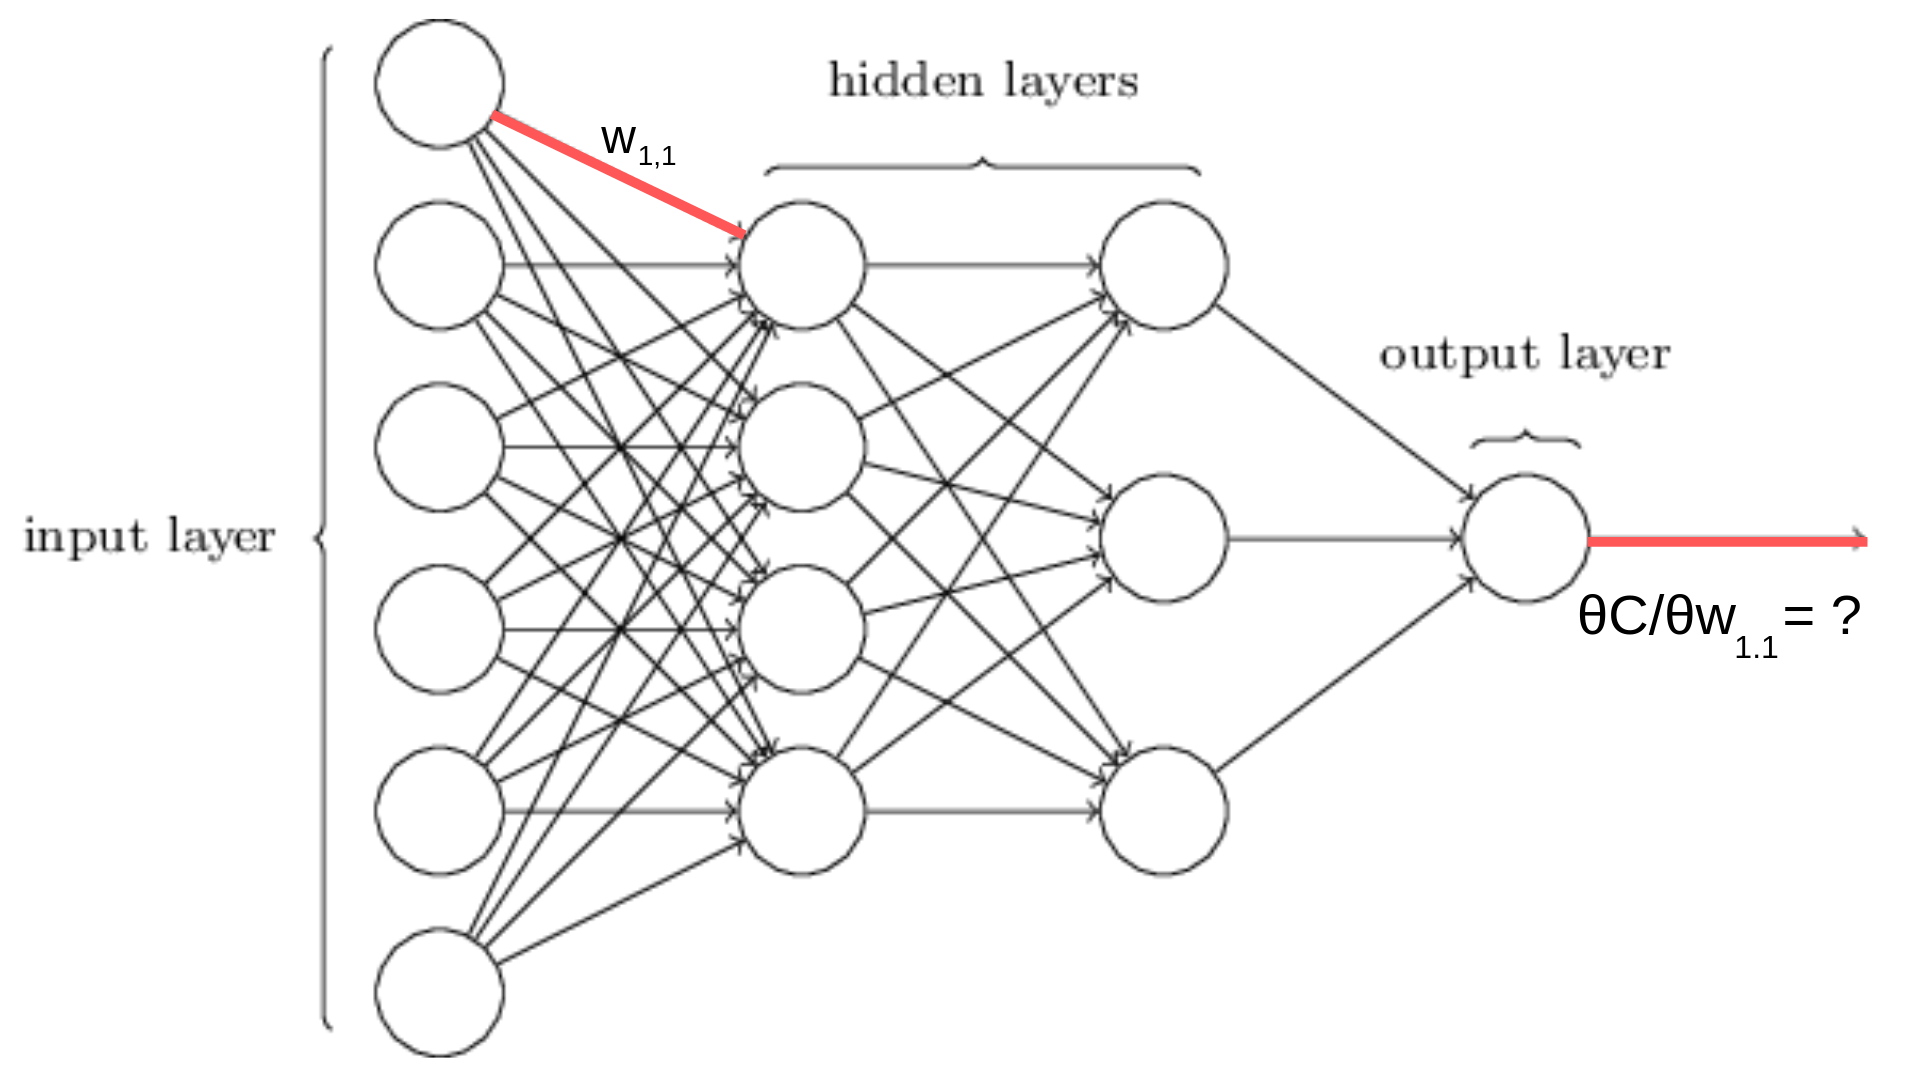
\includegraphics[width=.8\linewidth]{imgs/mlp_backprop}
  \end{figure}
\end{frame}

\begin{frame}
  \vspace{1cm}
  \textbf{Back Propagation:} PROPAGATE the errors BACK to the input weights! \\
  \begin{figure}
    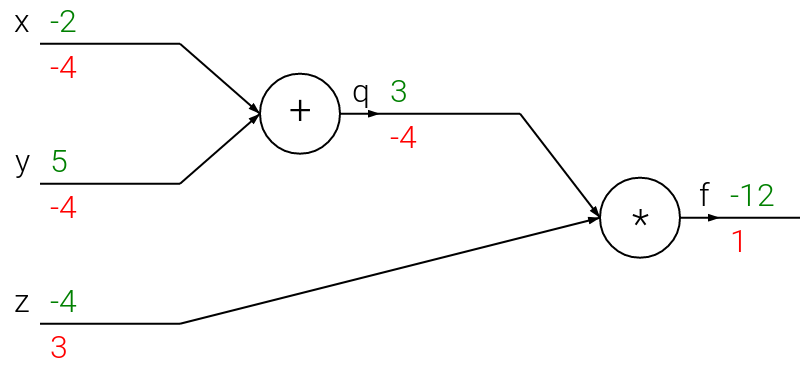
\includegraphics[width=.7\linewidth]{imgs/backprop_1}
  \end{figure}
  \textbf{Chain rule to the rescue!} \\
  $$\frac{\partial f}{\partial x} = \frac{\partial f}{\partial q} \frac{\partial q}{\partial x} =  \frac{\partial (q \cdot z)}{\partial q} \frac{\partial (x + y)}{\partial x} =
  z \cdot 1 = z = -4$$
  $$\frac{\partial f}{\partial z} = \frac{\partial (q \cdot z)}{\partial z} = q = 3$$
\end{frame}

\begin{frame}
  \vspace{0.6cm}
  \textbf{Sigmoid neurons - Sigmoid activation function} \\
  We want a small change in weight to cause only a small corresponding change in the output from the network. \\
  \textbf{Not possible with perceptrons!} - a small change in the weights or bias of any single perceptron in the network can sometimes cause the output of that perceptron to completely flip, say from 0 to 1
  \begin{figure}
    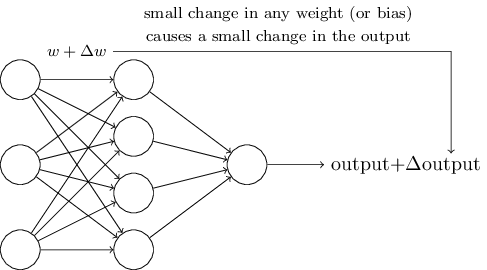
\includegraphics[width=.7\linewidth]{imgs/sigmoid_1}
  \end{figure}
\end{frame}

\begin{frame}
  \vspace{0.7cm}
  \begin{multicols}{2}
    The ouputs of the sigmoid neuron is NOT 0 or 1. \\
    $output = \sigma(w \cdot x + b)$, where $\sigma$ is the sigmoid function. \\
    $$\sigma(z) = \frac{1}{1 + e^{-z}} = \frac{1}{1 + exp(-\sum_j w_jx_j - b)}$$
    \columnbreak
    \begin{figure}
      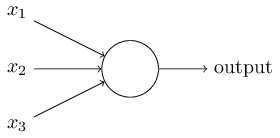
\includegraphics[width=.7\linewidth]{imgs/sigmoid_2}
    \end{figure}
  \end{multicols}

  \begin{figure}[ht]
  	\centering
  	\subfloat{%

  		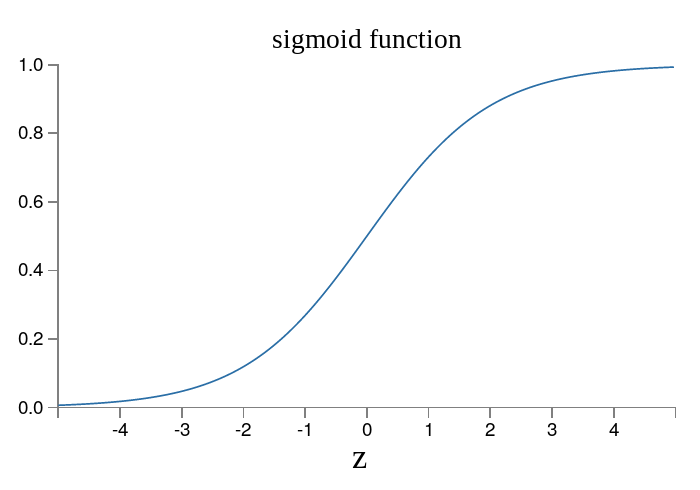
\includegraphics[width=0.45\linewidth]{imgs/ch-02-v4-06a}}%
  	\qquad
  	\subfloat{%
  		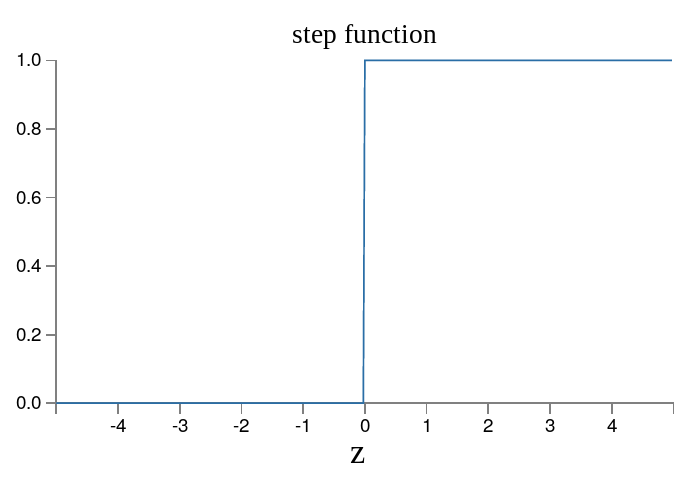
\includegraphics[width=0.45\linewidth]{imgs/ch-02-v4-06b}}%
  \end{figure}

\end{frame}

\begin{frame}
  \vspace{1cm}
  \begin{figure}
    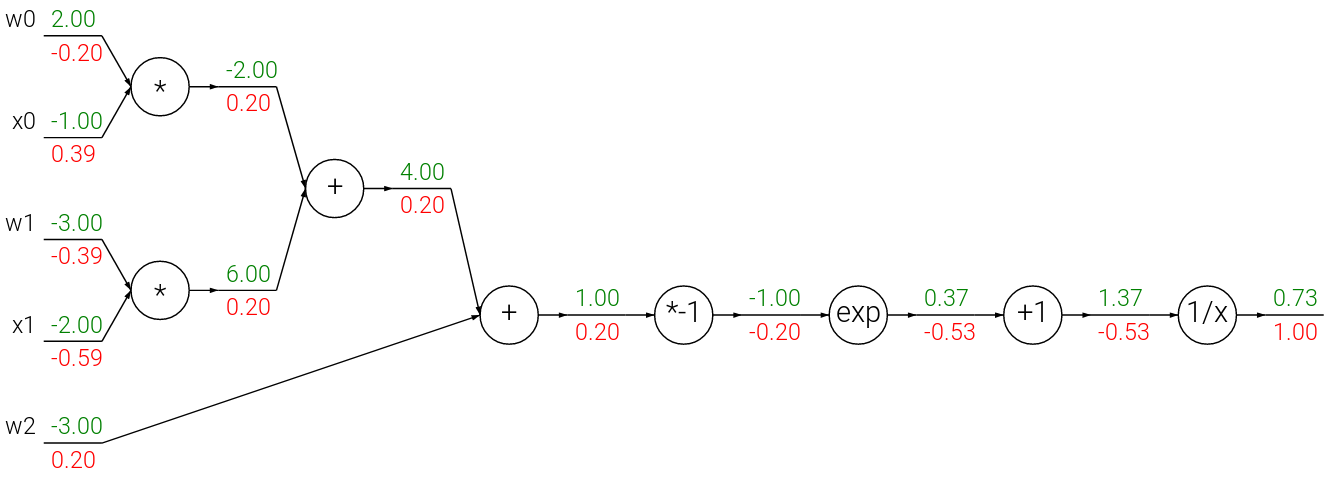
\includegraphics[width=1\linewidth]{imgs/backprop_2}
  \end{figure}
  $q = w_0 \cdot x_0,$ \quad $p = w_1 \cdot x_1,$ \quad $s = q + p,$ \quad $t = w_2 + s,$ \quad $r = -t,$ \quad $u = e^r,$ \quad $v = u + 1$ and $z = \frac{1}{v}$ \\
  \Large{$\frac{\partial z}{\partial w_0} = \frac{\partial z}{\partial v}\frac{\partial v}{\partial u}\frac{\partial u}{\partial r}\frac{\partial r}{\partial t}\frac{\partial t}{\partial s}\frac{\partial s}{\partial q}\frac{\partial q}{\partial w_0} = $} \\
  \small{$-0.53 \cdot 1 \cdot 0.37 \cdot (-1) \cdot 1 \cdot 1 \cdot  x_0 = -0.1961 \approx -0.20$}
\end{frame}

\begin{frame}
  \vspace{1cm}
  \begin{figure}
    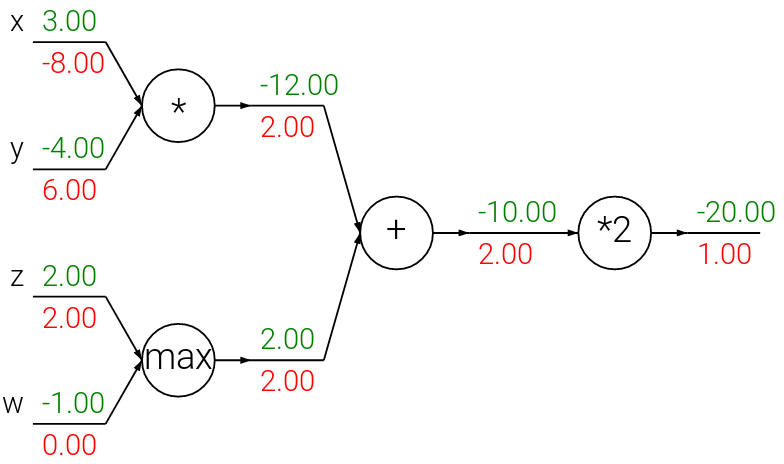
\includegraphics[width=1\linewidth]{imgs/backprop_3}
  \end{figure}
\end{frame}


\begin{frame}
  \vspace{1cm}
  softmax, \\
  NN as matrices, \\

  MNIST example keras (dense) \\

  overfitting / underfitting

\end{frame}

\begin{frame}
  Python script - draw/update boundaries while learning!!! \\
  https://cs.stanford.edu/people/karpathy/convnetjs/demo/classify2d.html \\
  1 neuron demo - gates, function approximation (y = 2x), house prices, etc \\
(gradient descent)
python demo - XOR problem (boundaries cant converge) \\
Linear model!!! meaning a straight line or a linear hyperplane

Linera regression learn the rules \\

\end{frame}

\begin{frame}
machine learning is all about a computer learning the patterns that distinguish things \\
map x to y example (y = x-1)
\end{frame}

\begin{frame}
  Laurence Moroney \\
traditional programming vs ML (rules + data = ans VS ans + data = rules) \\
the computer will figure out the rules \\
+ examples slides
\end{frame}

\begin{frame}
\href{https://news.psu.edu/story/429727/2016/10/04/research/artificial-intelligence-could-help-farmers-diagnose-crop-diseases}{Artificial intelligence could help farmers diagnose crop diseases} \\
%
\href{https://www.youtube.com/watch?v=NlpS-DhayQA}{TensorFlow: an ML platform for solving impactful and challenging problems} \\

TensorFlow: an ML platform for solving impactful and challenging problems [\href{https://www.youtube.com/watch?v=NlpS-DhayQA}{link}] \\

Let there be Color! [\href{http://iizuka.cs.tsukuba.ac.jp/projects/colorization/extra.html}{link}] \\

Let there be Color! [\href{https://github.com/satoshiiizuka/siggraph2016_colorization}{github}]

refs \\
\href{https://www.sciencedaily.com/terms/artificial_intelligence.htm}{AI - Def.}


\end{frame}

\end{document}
